\begin{savequote}[45mm]
\ascii{Any fool can write code that a computer can understand. Good programmers write code that humans can understand.}
\qauthor{\ascii{- Martin Flower}}
\end{savequote}

\chapter{破冰之旅} 
\label{ch:ice-breaker}

\begin{content}

在开始探究\tf{}内核之前,亲自动手实践模型的训练,熟悉模型训练的基本方法和调优技术,对于理解后续章节的内容将大有裨益。通过本文学习和实践,将了解到如何构建并训练出能够识别手写数字的神经网络\footnote{ 本章内容摘自\ascii{Martin G\"{o}rner}在\ascii{Codelabs}上发表的文章:\href{https://codelabs.developers.google.com/codelabs/cloud-tensorflow-mnist}{Tensorflow and deep learning, without a PhD},经由\ascii{Martin G\"{o}rner}同意,授权该文章在本书中发表。}。

在开始时,尝试使用单层感知器模型,进而尝试使用多层感知器模型,最后尝试使用卷积神经网络。并在训练过程中,介绍了算法调优的一些常用技术,包括选择更好的激活函数,应用学习速率衰减的技术,实施\ascii{Dropout}技术等。最终,将模型的准确率提升至\ascii{99%}以上。

在介绍每一种网络模型之前,将简单给出该模型的算法理论知识,帮助大家更好地理解程序的内容。但是,本书不是介绍机器学习算法的专业书籍,如需了解更多相关算法内容,请查阅相关文献和论文。

\end{content}

\section{问题提出}

\begin{content}

本章使用\ascii{MNIST}数据集完成手写数字的网络模型训练,它包含了\ascii{60000}个训练样本数据;其中,包括\ascii{10000}个测试样本数据。如\refig{mnist-x}所示,对于任意一个样本数据$x$,使用$28 \times 28$像素的数字矩阵表示。为了简化,将$28 \times 28$的矩阵实施扁平化处理,得到长度为\ascii{784}的一维向量。

\begin{figure}[H]
\centering
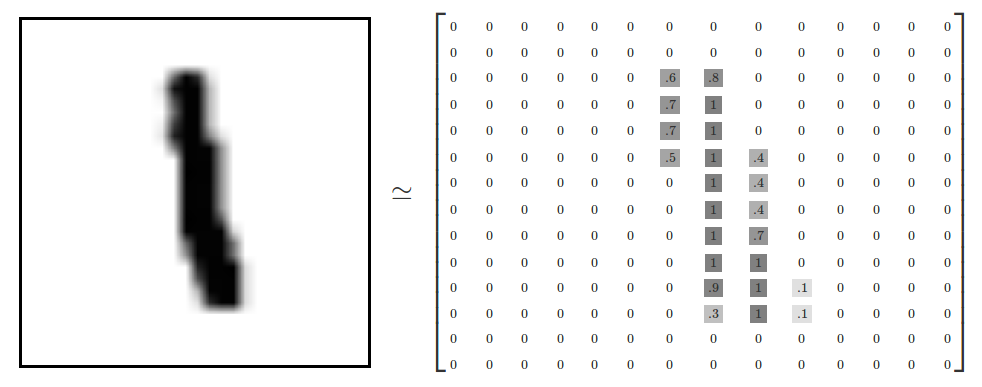
\includegraphics[width=0.9\textwidth]{figures/mnist-x.png}
\caption{MNIST样本数据表示}
 \label{fig:mnist-x}
\end{figure}

\subsection{样本数据集}

因此,在\ascii{MNIST}训练数据集中,\code{mnist.train.images}是一个\code{[60000, 784]}的二维矩阵。其中,矩阵中每一个元素,表示图片中某个像素的强度值,其值介于\ascii{0}和\ascii{1}之间。如\refig{mnist-train-xs}所示。

\begin{figure}[H]
\centering
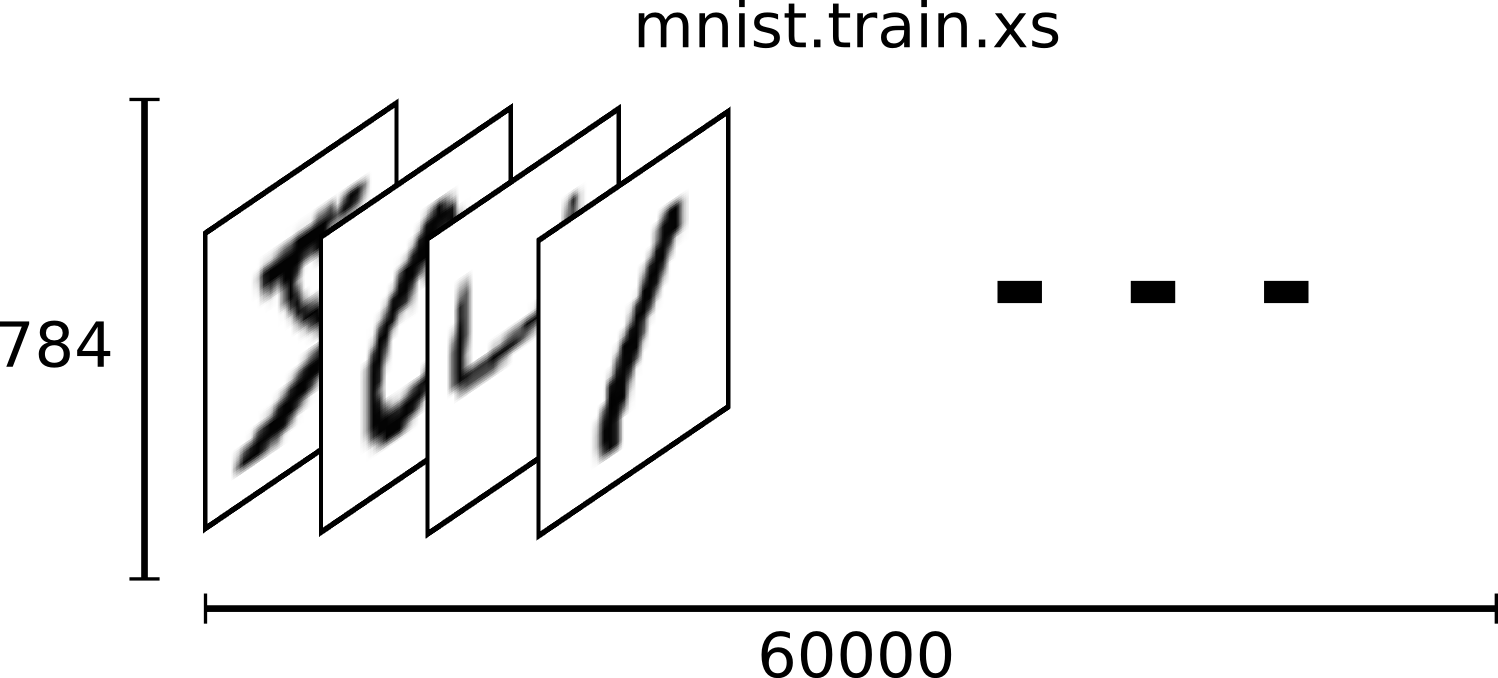
\includegraphics[width=0.9\textwidth]{figures/mnist-train-xs.png}
\caption{MNIST训练数据集:输入数据集}
 \label{fig:mnist-train-xs}
\end{figure}

相对应地,\ascii{MNIST}数据集的标签是介于\ascii{0}到\ascii{9}的数字,\code{mnist.train.labels}是一个\code{[60000, 10]}的二维矩阵,其中每一行是一个\ascii{\quo{one-hot}}向量。如\refig{mnist-train-ys}所示。

\begin{figure}[H]
\centering
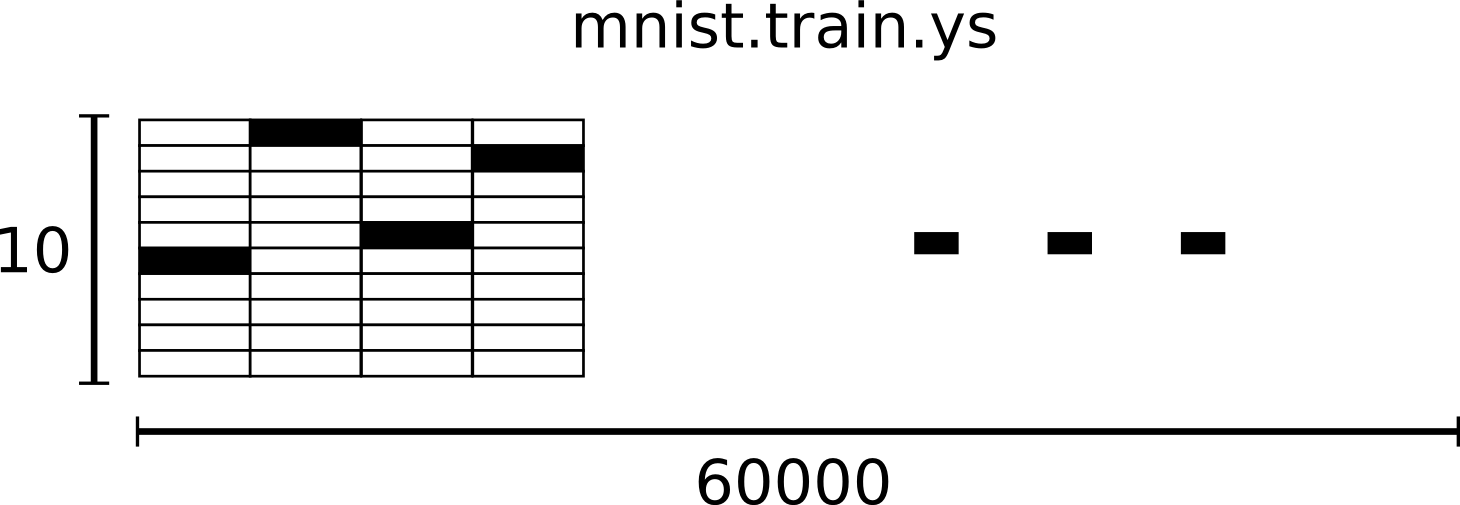
\includegraphics[width=0.9\textwidth]{figures/mnist-train-ys.png}
\caption{MNIST训练数据集:标签数据集}
 \label{fig:mnist-train-ys}
\end{figure}

\subsection{图示说明}

\begin{content}

为了更好地可视化整个训练过程,使用\ascii{matplotlib}工具包绘制了\ascii{5}种类型的画板。如\refig{mnist-training-digits}所示,表示一个\ascii{mini-batch}的训练样本数据集。其中,\code{batch\_size = 100},白色背景表示数字被正确识别;而红色背景表示数字被误分类,手写数字的左侧标识了正确的标签值,而右侧标识了错误的预测值。

\ascii{MNIST}拥有\ascii{50000}个训练样本,如果\code{batch\_size}为\ascii{100},则需要迭代\ascii{500}次才能完整地遍历一次训练样本数据集,常称为一个\ascii{epoch}周期。

\begin{remark}
本章示例代码未使用\ascii{TensorBoard},而是用了\ascii{matplotlib},在训练时可以实时观察误差和精度的曲线变化。
\end{remark}

\begin{figure}[H]
\centering
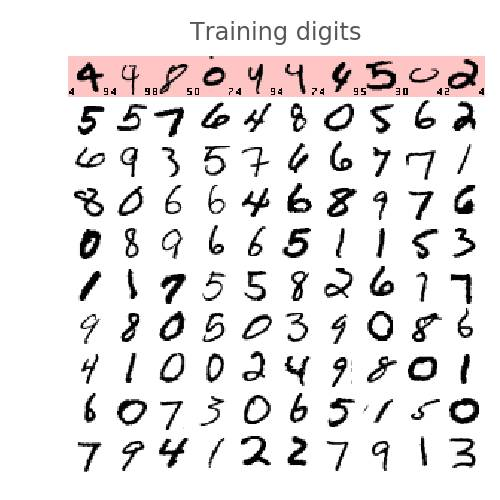
\includegraphics[width=0.6\textwidth]{figures/mnist-training-digits.jpeg}
\caption{一次mini-batch的训练样本数据集,其中\code{batch\_size=100}}
 \label{fig:mnist-training-digits}
\end{figure}

如\refig{mnist-test-digits}所示,\ascii{MNIST}使用了规模为\ascii{10000}的测试样本数据集测试模型的当前精度。其中,左侧表示目前模型的大致精度;同样地,白色背景表示数字被正确识别;而红色背景表示数字被误分类,手写数字的左侧标识了正确的标签值,而右侧标识了错误的预测值。

\begin{figure}[H]
\centering
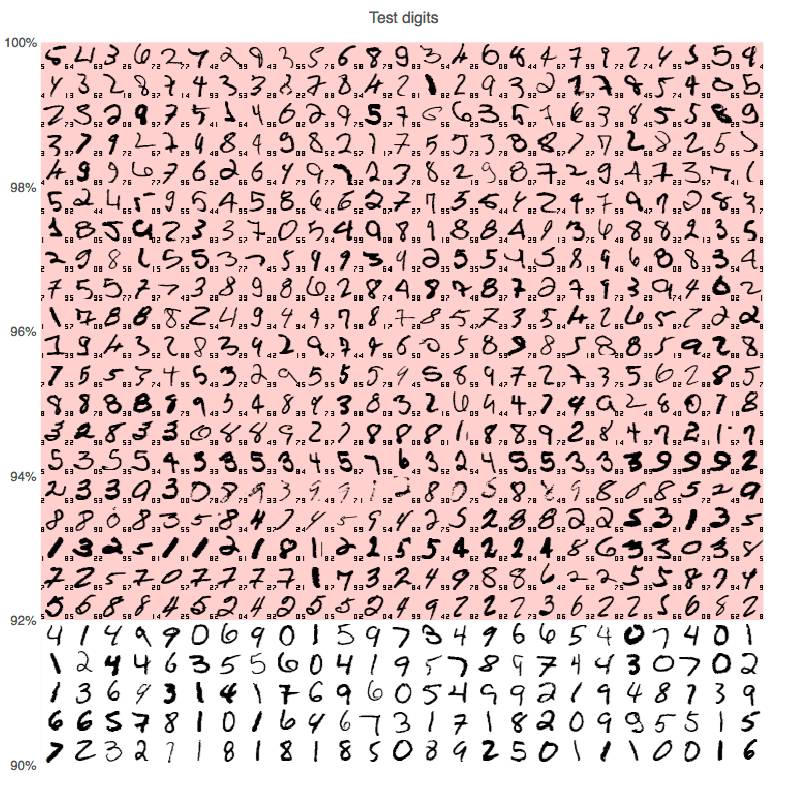
\includegraphics[width=0.6\textwidth]{figures/mnist-test-digits.jpeg}
\caption{当前的模型精度:基于测试样本数据集}
 \label{fig:mnist-test-digits}
\end{figure}

如\refig{mnist-cross-entropy-loss-fig}所示,使用交叉熵函数量化预测值与标签值之前的误差。其中,\ascii{x}轴表示迭代的次数,\ascii{y}轴表示损失值。另外,基于训练样本数据集,损失值的曲线抖动较大;而基于测试样本数据集,损失值的曲线抖动较小。

\begin{figure}[H]
\centering
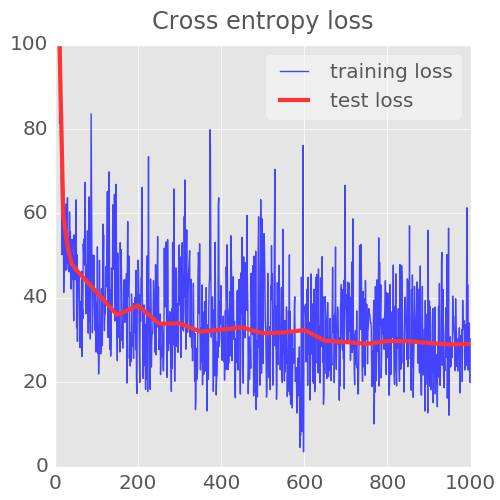
\includegraphics[width=0.6\textwidth]{figures/mnist-cross-entropy-loss-fig.jpeg}
\caption{训练和测试的交叉熵损失}
 \label{fig:mnist-cross-entropy-loss-fig}
\end{figure}

如\refig{mnist-accuracy-fig}所示,可以实时计算得到模型在当前训练数据集和测试集上的精度。其中,\ascii{x}轴表示迭代的次数,\ascii{y}轴表示精度值。同理,基于训练样本数据集,精度曲线抖动较大;而基于测试样本数据集,精度曲线抖动较小。

\begin{figure}[H]
\centering
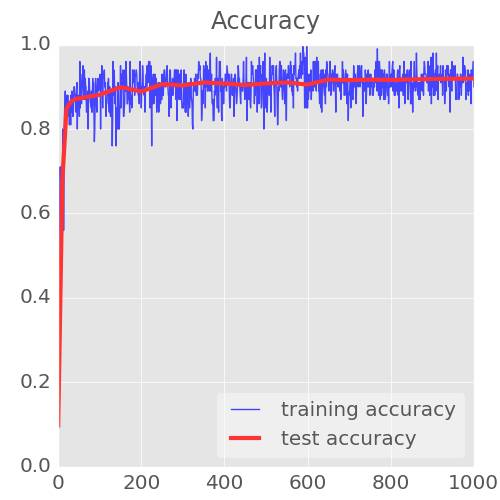
\includegraphics[width=0.6\textwidth]{figures/mnist-accuracy-fig.jpeg}
\caption{训练和测试的精度}
 \label{fig:mnist-accuracy-fig}
\end{figure}

如\refig{mnist-weight-fig}所示,对于模型的每一个训练参数(包括偏置),可以统计得到其对应的数值分布图。当模型不能收敛时,参数的数值分布图能够给出有帮助的提示信息。

\begin{figure}[H]
\centering
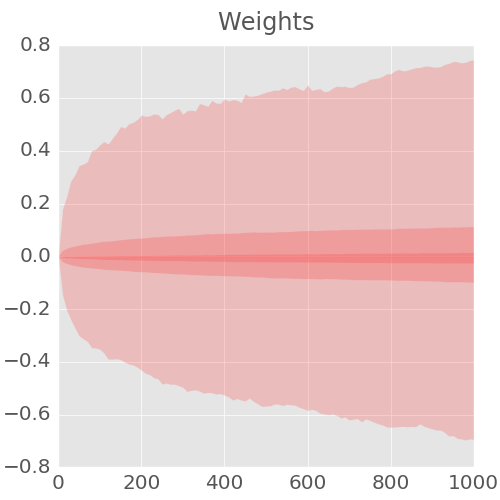
\includegraphics[width=0.6\textwidth]{figures/mnist-weight-fig.png}
\caption{权重分布图}
 \label{fig:mnist-weight-fig}
\end{figure}

\end{content}

\section{单层感知器}

\begin{content}

首先,尝试构建\ascii{10}个神经元的单层感知器。如\refig{mnist-slp}所示,对于诸如手写数字识别的多分类问题,理论上常使用\ascii{softmax}的激活函数。

\begin{figure}[H]
\centering
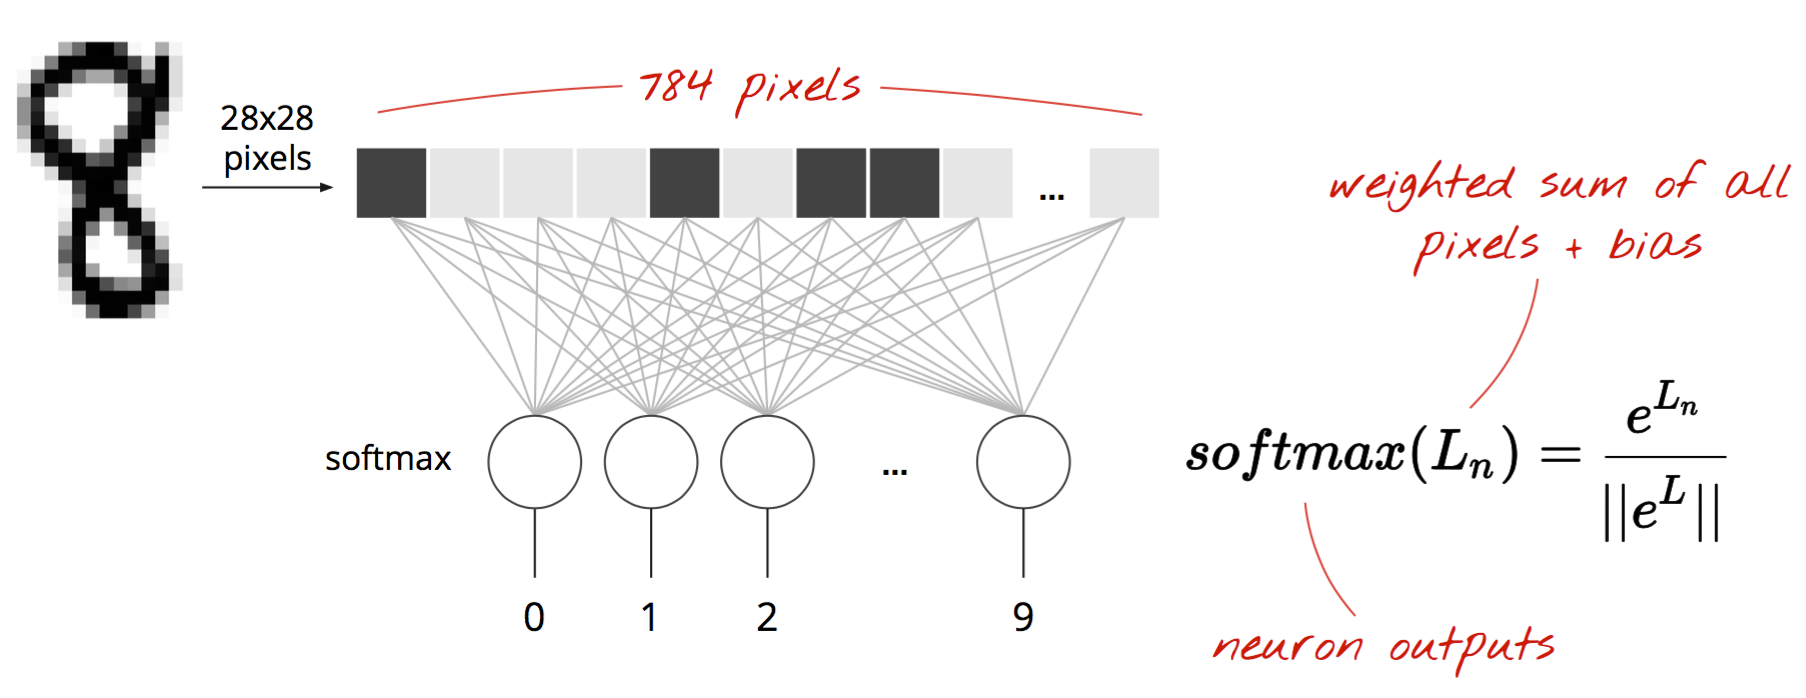
\includegraphics[width=0.8\textwidth]{figures/mnist-slp.png}
\caption{单层感知器}
 \label{fig:mnist-slp}
\end{figure}

\subsection{理论基础}

理论上,\ascii{softmax}回归是\ascii{logistic}回归的广义扩展。其中,\ascii{logistic}回归是为了解决二分类问题,即$y \in \{ 0,1\}$;而\ascii{softmax}回归是为了解决$ k $分类问题,即$y \in \{ 1,2,...,k\}$。

\subsubsection{符号定义}

为了形式化地描述\ascii{softmax}回归问题,此处定义了一些常用符号。

 \begin{itemize}
   \item \ascii{训练样本集}: $ S = \{ ({x^{(i)}},{y^{(i)}});i = 1,2,...,m\} $
   \item \ascii{第$i$个训练样本}: $ ({x^{(i)}},{y^{(i)}}) $
   \item \ascii{样本输入}: $ x = ({x_1},{x_2},...,{x_n})^{T}  \in {\mathbb{R}^n} $
   \item \ascii{样本标签(one-hot)}: $ y = ({y_1},{y_2},...,{y_k})^{T} \in {\mathbb{R}^k} $
   \item \ascii{权重}: $ W \in {\mathbb{R}^{n \times k}} $   
   \item \ascii{偏置}: $ b \in {\mathbb{R}^k} $   
   \item \ascii{softmax函数}: $ 
softmax {(z_i)} = \tfrac{{{e^{{z_i}}}}}{{\sum\limits_{j = 1}^k {{e^{{z_j}}}} }}  \quad i = 1,2,...,k
$
 \end{itemize}

\subsubsection{softmax函数}

如\refig{softmax}所示,模型先求取线性加权和$z$,然后求取$e^z$,最后再实施归一化操作。

\begin{figure}[H]
\centering
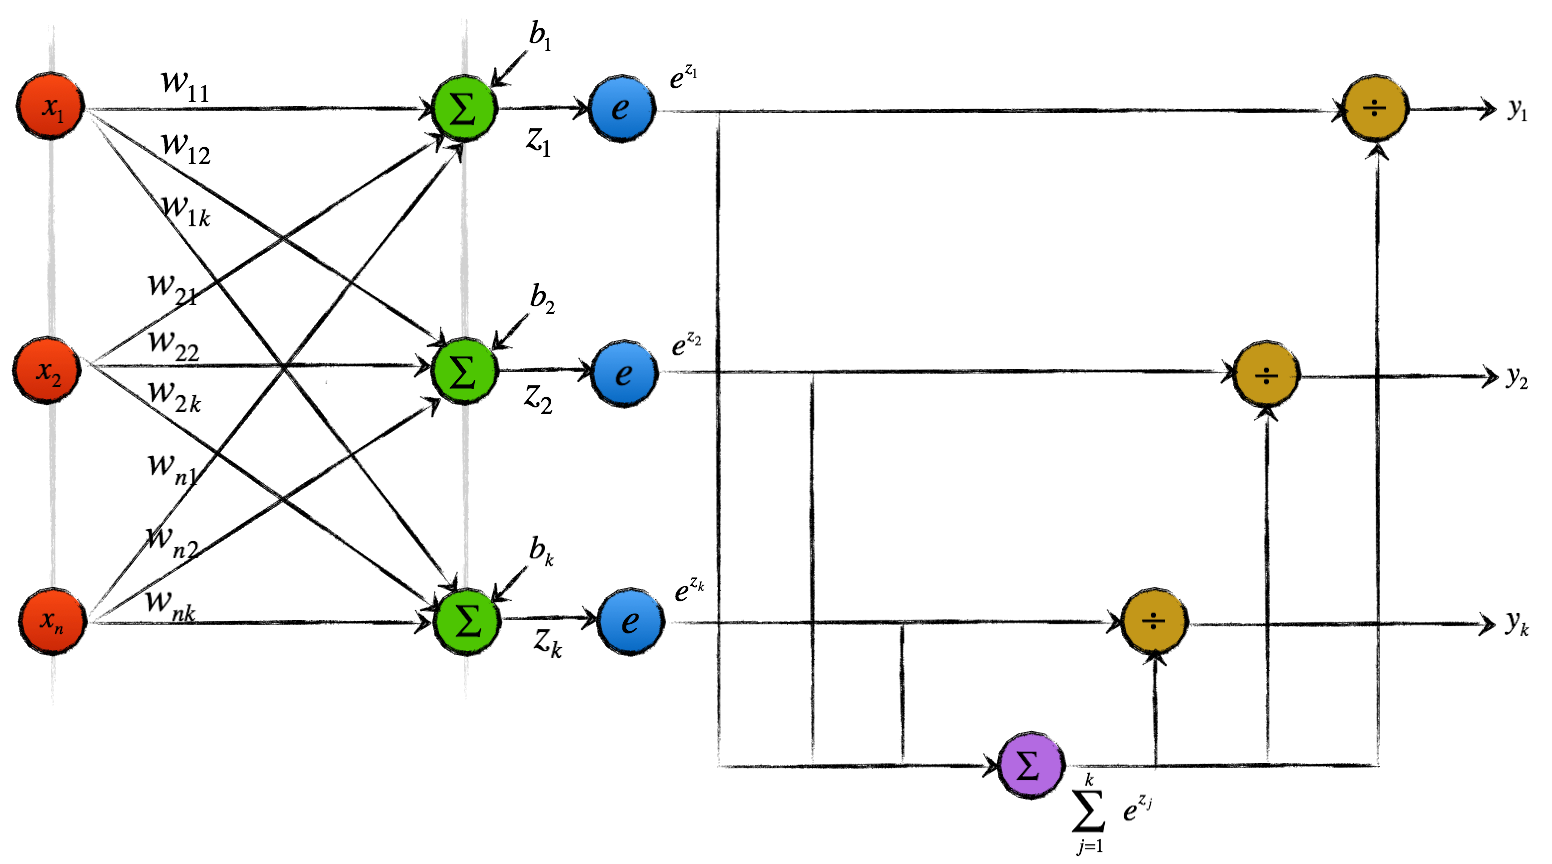
\includegraphics[width=0.8\textwidth]{figures/softmax.png}
\caption{softmax函数}
 \label{fig:softmax}
\end{figure}

\subsubsection{权重与偏置}

权重$W$为一个$n \times k$的二维矩阵。

\[
W = \left( {{W_1},{W_2},...,{W_k}} \right) = \left( {\begin{array}{*{20}{c}}
  {{w_{11}}}& \ldots &{{w_{1k}}} \\ 
   \vdots & \ddots & \vdots  \\ 
  {{w_{n1}}}& \cdots &{{w_{nk}}} 
\end{array}} \right) \in {\mathbb{R}^{n \times k}}
\]

其中,$W_j$是一个长度为$n$的向量。

\[
{W_j} = {\left( {{w_{1j}},{w_{2j}},...,{w_{nj}}} \right)^T} \in {\mathbb{R}^n}, j = 1,2,...,k \\
\]

而偏置$b$是一个长度为$k$的\ascii{\quo{one-hot}}向量。

\[
b = {({b_1},{b_2},...,{b_k})^T} \in {\mathbb{R}^k}
\]

\subsubsection{模型定义}

多分类问题的单层感知器模型,使用\ascii{softmax}激活函数,可以如此定义。

\[\begin{aligned}
  y =  & {h_{W,b}}(x) = softmax (z) = softmax ({W^T}x + b) \\ 
   =  & {\left( {{y_1},{y_2},...,{y_k}} \right)^T} \\ 
   =  & \frac{1}{{\sum\limits_{j = 1}^k {{e^{{z_j}}}} }}{\left( {{e^{{z_1}}},{e^{{z_2}}},...,{e^{{z_k}}}} \right)^T} \\ 
   =  & \frac{1}{{\sum\limits_{j = 1}^k {{e^{W_j^Tx + {b_j}}}} }}{\left( {{e^{W_1^Tx + {b_1}}},{e^{W_2^Tx + {b_2}}},...,{e^{W_k^Tx + {b_k}}}} \right)^T} \ 
\end{aligned} \]

其中,对于任意给定的样本$ (x, y) \in S $,$ z_i $表示$W_i^Tx+b_i$的线性加权和,而$y_i(i=1,2,...,k)$表示将其划归为类$i$的概率。

\[\begin{gathered}
  P\left( {y = i|x;W,b} \right) = \frac{{{e^{W_i^Tx + b_i}}}}{{\sum\limits_{j = 1}^k {{e^{W_j^Tx + b_j}}} }} \hfill \\
  i = 1,2,...,k \hfill \\ 
\end{gathered} \]


\subsubsection{交叉熵函数}

基于样本数据集$ S = \{ ({x^{(i)}},{y^{(i)}});i = 1,2,...,m\} $,交叉熵损失函数可以如此定义。

\[\begin{aligned}
  J(W,b) =  &  - \frac{1}{m}\sum\limits_{i = 1}^m {{y^{(i)}}\log \left( {{{\widehat y}^{(i)}}} \right)}  \\ 
   =  &  - \frac{1}{m}\sum\limits_{i = 1}^m {\sum\limits_{j = 1}^k {y_j^{(i)}\log \left( {\widehat y_j^{(i)}} \right)} }  \\
\end{aligned} \]

\ascii{softmax}多分类问题,就是求取最优解$(W^*,b^*)$,使得

\[W^*,b^* = \mathop {\arg \min }\limits_{W,b} J(W,b)\]

\subsubsection{计算梯度}

对于任意一个样本$ (x,y) \in S $,可以推导出$ J(W,b) $相对于$ W $与$ b $的梯度公式。

\[\begin{aligned}
  {\nabla _W}J\left( {W,b;x,y} \right) =  & \left( {\widehat y - y} \right)x \\ 
  {\nabla _b}J\left( {W,b;{x^{(i)}},{y^{(i)}}} \right) =  & \left( {\widehat y - y} \right) \\ 
\end{aligned} \]


\subsubsection{参数更新}

对于训练样本数据$ S $,根据$W, b$的梯度公式,完成本次迭代的参数更新。

\[\begin{aligned}
  W \leftarrow  & W - \alpha \frac{{\sum\limits_{i = 1}^m {{\nabla _W}J\left( {W,b;{x^{(i)}},{y^{(i)}}} \right)} }}{m} \\ 
  b \leftarrow  & b - \alpha \frac{{\sum\limits_{i = 1}^m {{\nabla _b}J\left( {W,b;{x^{(i)}},{y^{(i)}}} \right)} }}{m} \\ 
\end{aligned} \]

\subsection{定义模型}

接下来,使用\tf{}完成该模型的搭建和训练。需要注意的是,理论上的公式与\tf{}具体实现存在微妙的差异。理论上,公式中的$x$常表示一个样本,但\tf{}中的\code{x}常表示一个\ascii{mini-batch}的样本数据集。因此,使用\tf{}设计网络模型时,需要特别关注各个张量大小的变化是否符合预期。

\subsubsection{输入和标签}

首先,使用\code{tf.placeholder}分别定义训练样本的输入和标签。

\begin{leftbar}
\begin{python}
x = tf.placeholder(tf.float32, [None, 28, 28, 1])
t = tf.placeholder(tf.float32, [None, 10])
\end{python}
\end{leftbar}

\code{tf.placeholder}定义了一个占位的\ascii{OP}。\code{None}表示未确定的样本数目,此处表示\code{batch\_size}的大小;当\code{Session.run}时,将通过\code{feed\_dict}的字典提供一个\ascii{mini-batch}的样本数据集,从而自动推导出\code{tf.placeholder}的大小。

另外,每张图片使用$ 28 \times 28 \times 1 $的三维数据表示(灰度为\ascii{1})。为了简化问题,此处将输入的样本数据扁平化,将其变换为长度为\ascii{784}的一维向量。其中,\ascii{-1}表示\ascii{mini-batch}的样本数目,由运行时自动推演其大小。

\begin{leftbar}
\begin{python}
x = tf.reshape(x, [-1, 784])
\end{python}
\end{leftbar}

\subsubsection{定义变量}

然后,使用\code{tf.Variable}定义模型参数。定义训练参数时,必须指定参数的初始化值;训练参数将根据初始值,自动推演数据的类型,及其大小。

\begin{leftbar}
\begin{python}
w = tf.Variable(tf.zeros([784, 10]))
b = tf.Variable(tf.zeros([10]))
\end{python}
\end{leftbar}

此外,变量在使用之前,必须完成初始化。此处,\code{init\_op}将初始化所有全局的训练参数。

\begin{leftbar}
\begin{python}
init_op = tf.global_variables_initializer()
\end{python}
\end{leftbar}

\subsubsection{模型定义}

接下来,便可以很容易地得到多分类问题的单层感知器模型。

\begin{leftbar}
\begin{python}
y = tf.nn.softmax(tf.matmul(x, w) + b)
\end{python}
\end{leftbar}

如\refig{mnist-linear-sum}所示,首先计算\code{x}与\code{w}的矩阵乘法,让后将\code{b}广播(\ascii{broadcast})到矩阵的每一行相加,最终得到训练参数的线性加权和。

\begin{figure}[H]
\centering
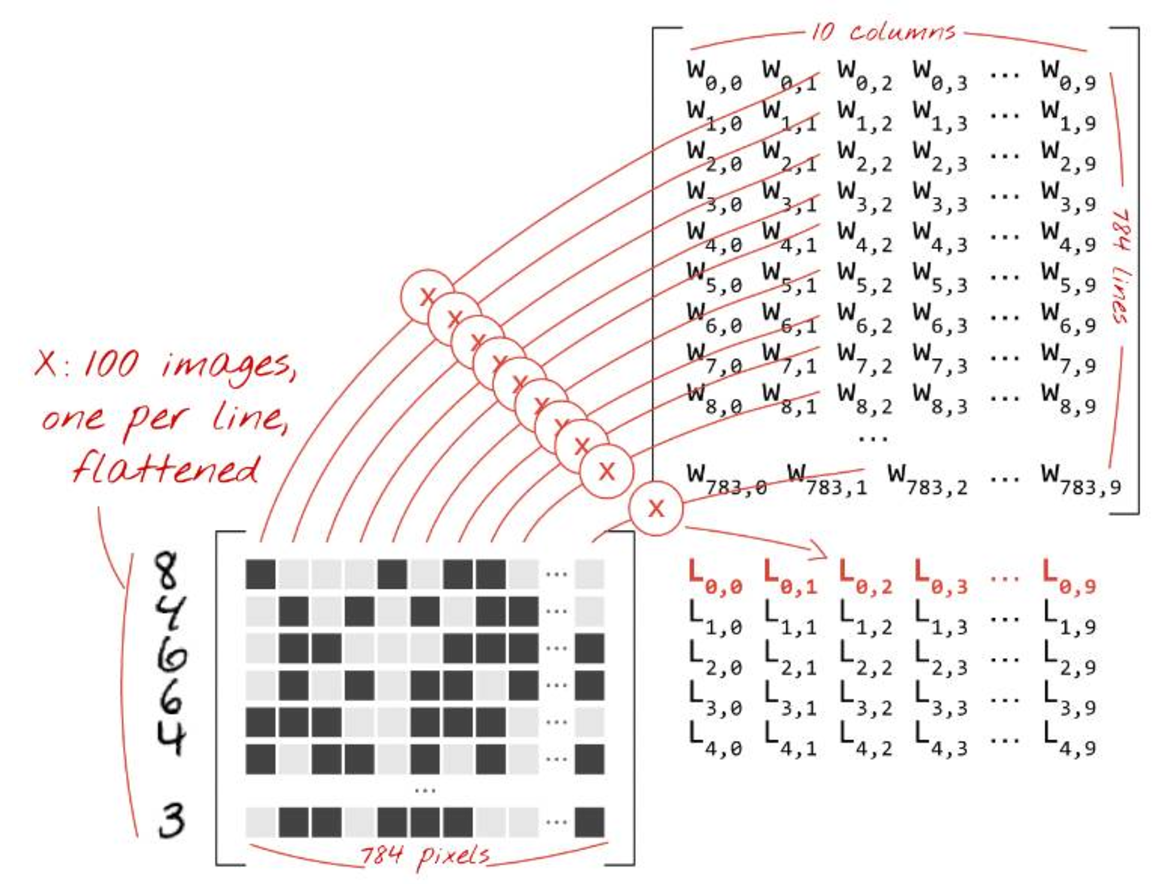
\includegraphics[width=0.8\textwidth]{figures/mnist-linear-sum.png}
\caption{线性加权和}
 \label{fig:mnist-linear-sum}
\end{figure}

如\refig{mnist-softmax}所示,\ascii{softmax}将逐行实施运算,最终,\code{y}的大小为\code{[100, 10]}。

\begin{figure}[H]
\centering
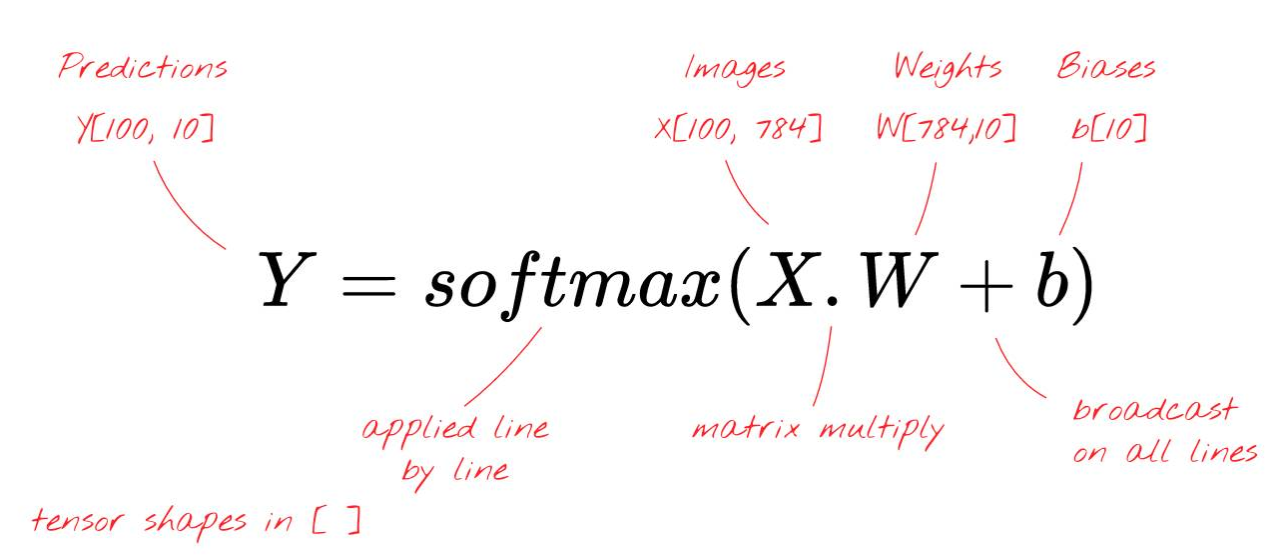
\includegraphics[width=0.8\textwidth]{figures/mnist-softmax.png}
\caption{激活函数:softmax}
 \label{fig:mnist-softmax}
\end{figure}

\subsubsection{损失函数}

对于多分类问题,可以使用交叉熵的损失函数。

\begin{leftbar}
\begin{python}
cross_entropy = -tf.reduce_sum(t * tf.log(y))
\end{python}
\end{leftbar}

如\refig{mnist-cross-entropy}所示,\code{t}和\code{y}的大小都为\code{[100, 10]};特殊地,\code{t}的每一行都是一个\quo{\ascii{one-hot}}向量。

对\code{y}实施\code{tf.log}操作,也将得到一个大小为\code{[100, 10]}的矩阵。然后,\code{t}与\code{tf.log(y)}逐位相乘(并非矩阵相乘),也将得到大小为\code{[100, 10]}的矩阵。最终,\code{tf.reduce\_sum}将矩阵中所有元素相加,得到一个标量(\ascii{scalar})值。

\begin{figure}[H]
\centering
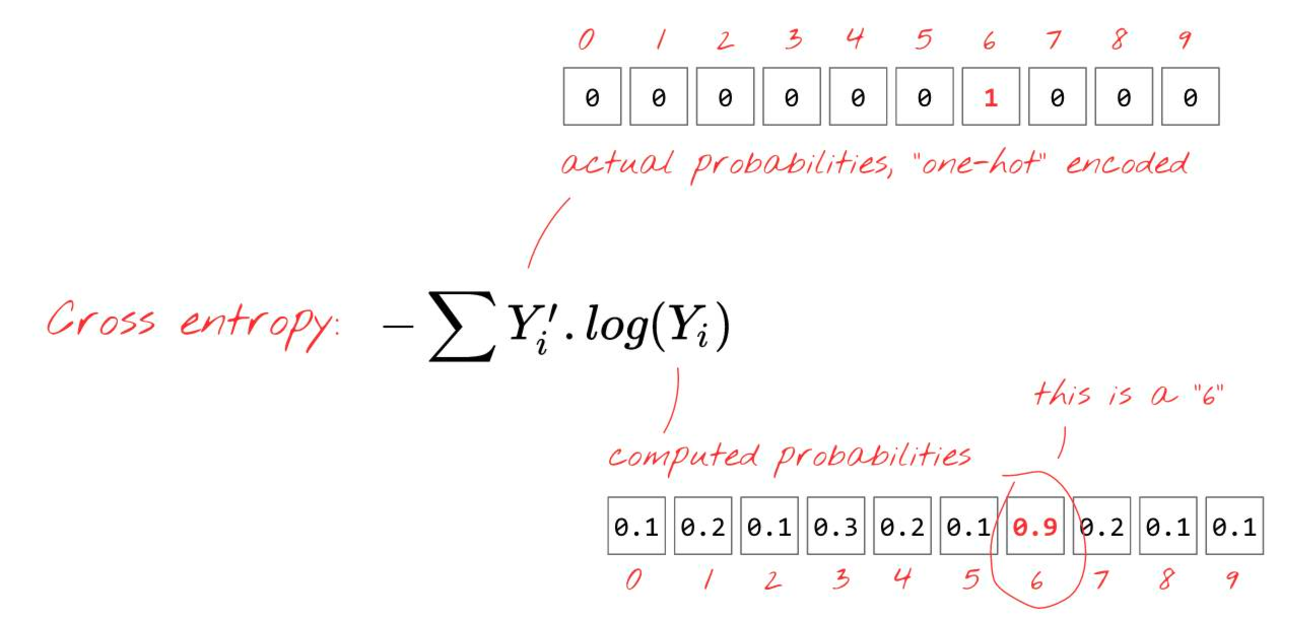
\includegraphics[width=0.8\textwidth]{figures/mnist-cross-entropy.png}
\caption{交叉熵损失函数}
 \label{fig:mnist-cross-entropy}
\end{figure}

\subsubsection{精度}

\code{tf.argmax(y,1)}将按第\ascii{1}个维度计算最大值的索引。既按照$ y_{100 \times 10} $的每一行,计算得到在每一行中最大值的的索引值。因此,\code{tf.argmax(y,1)}将得到大小为\code{[100, 1]}的矩阵,或大小为\ascii{100}的向量。同样地,\code{tf.argmax(t,1)}也是一个大小为\ascii{100}的向量。

然后,使用\code{tf.equal}将它们逐元素(\ascii{element-wise})进行相等性比较,得到大小为\ascii{100}的布尔向量。为了计算精度,先将布尔向量转别为数值向量,最终求取该数值向量的均值。

\begin{leftbar}
\begin{python}
is_correct = tf.equal(tf.argmax(y,1), tf.argmax(t,1))
accuracy = tf.reduce_mean(tf.cast(is_correct, tf.float32))
\end{python}
\end{leftbar}

\subsection{优化算法}

接下来,使用梯度下降算法实现交叉熵损失函数的最小化。其中,\code{learning\_rate}表示学习速率,描述参数更新的快慢和步伐大小,是一个典型的超参。

\begin{leftbar}
\begin{python}
optimizer = tf.train.GradientDescentOptimizer(learning_rate=0.003)
train_step = optimizer.minimize(cross_entropy)
\end{python}
\end{leftbar}

如\refig{mnist-gd}所示,可以将损失函数比作一座山,登山者试图寻找最佳的行动方案达到山谷。登山者站在某个山坡上环顾四周,决定沿梯度的反方向向下走一小步,直到达到局部最优。

当实施梯度下降更新算法时,初始点不同,获得的最小值也不同,因此梯度下降求得的只是局部最小值。另外,越接近最小值时,下降速度越慢。下降的步伐大小也非常重要,如果太小,则找到函数最小值的速度就很慢;如果太大,则可能会越过极值点。

\begin{figure}[H]
\centering
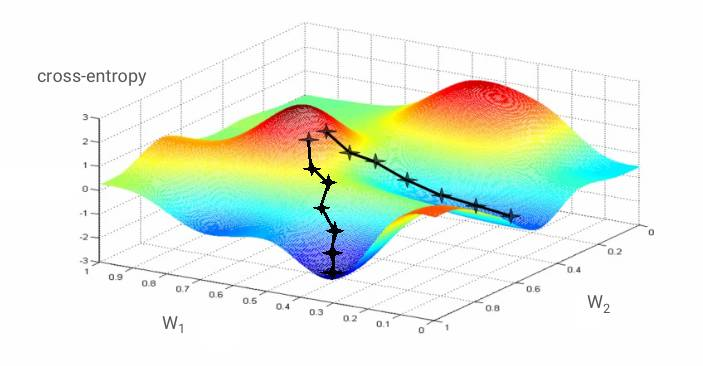
\includegraphics[width=0.8\textwidth]{figures/mnist-gd.jpeg}
\caption{梯度下降算法}
 \label{fig:mnist-gd}
\end{figure}

\subsection{训练模型}

在此之前,\tf{}仅构造计算图,并没有启动计算图的执行。接下来,客户端创建一个会话,建立与本地或远端计算设备集的通道,启动计算图的执行过程。

首先,完成训练参数的初始化。通过运行模型参数的初始化子图,并发地执行各个训练参数的初始化器,将初始值就地修改到相应的训练参数内。

\begin{leftbar}
\begin{python}
with tf.Session() as sess:
  sess.run(init_op)
\end{python}
\end{leftbar}

然后,开始迭代地执行\code{train\_step},完成模型的一次迭代训练。其中,每\ascii{100}次迭代,计算当前模型在训练数据集及测试数据集的精度和损失。

\begin{leftbar}
\begin{python}
with tf.Session() as sess:
  for step in range(1000):
    batch_xs, batch_ys = mnist.train.next_batch(100)        
    sess.run(train_step, feed_dict={x: batch_xs, t: batch_ys})
    
    if step % 100 == 0:
      acc, loss = sess.run([accuracy, cross_entropy], 
        feed_dict={x: batch_xs, t: batch_ys})
      acc, loss = sess.run([accuracy, cross_entropy], 
        feed_dict={x: mnist.test.images, t: mnist.test.labels}) 
\end{python}
\end{leftbar}

据统计,经过\ascii{1000}次迭代,可得到大约\percent{92}的精度。

\begin{figure}[H]
\centering
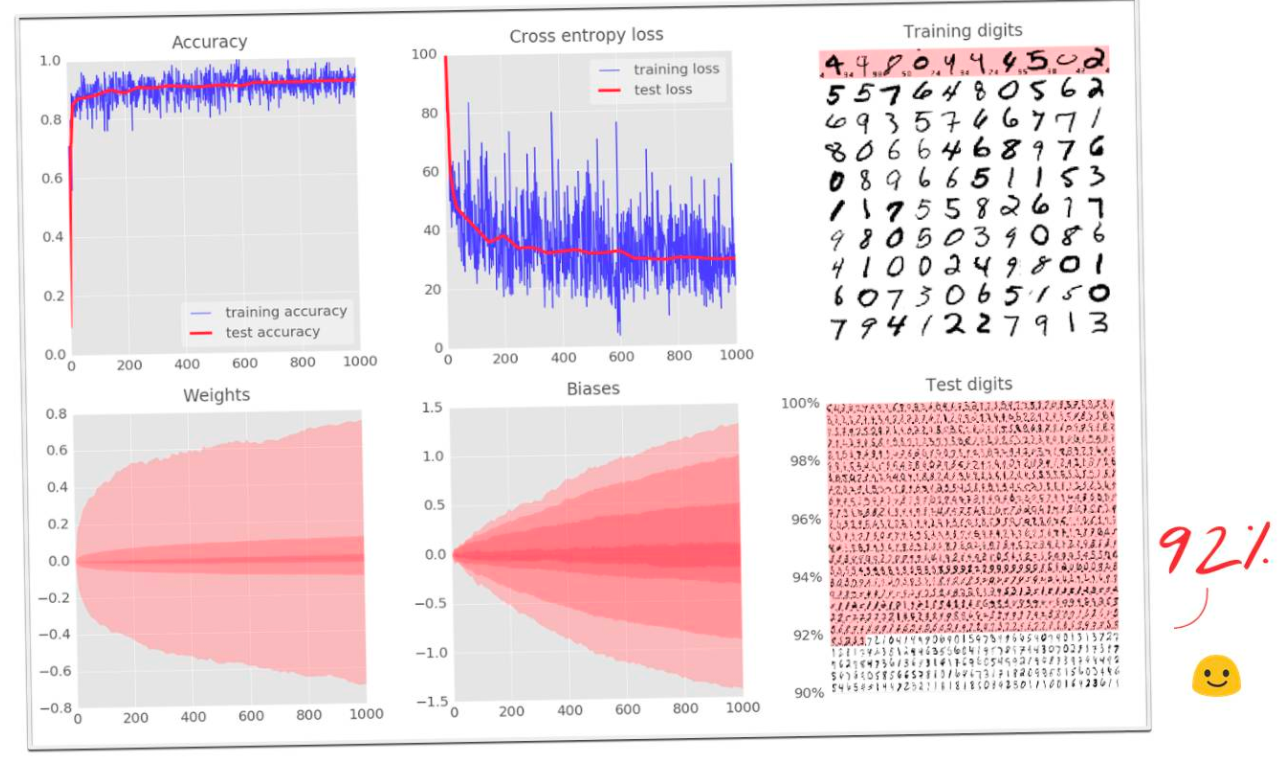
\includegraphics[width=0.8\textwidth]{figures/mnist-slp-accuracy.png}
\caption{可视化:单层感知器,运行1000次step}
 \label{fig:mnist-slp-accuracy}
\end{figure}

\end{content}

\section{多层感知器}

\begin{content}

为了进一步提高精度,接下来尝试搭建\ascii{5}层的多层感知器模型。

\begin{figure}[H]
\centering
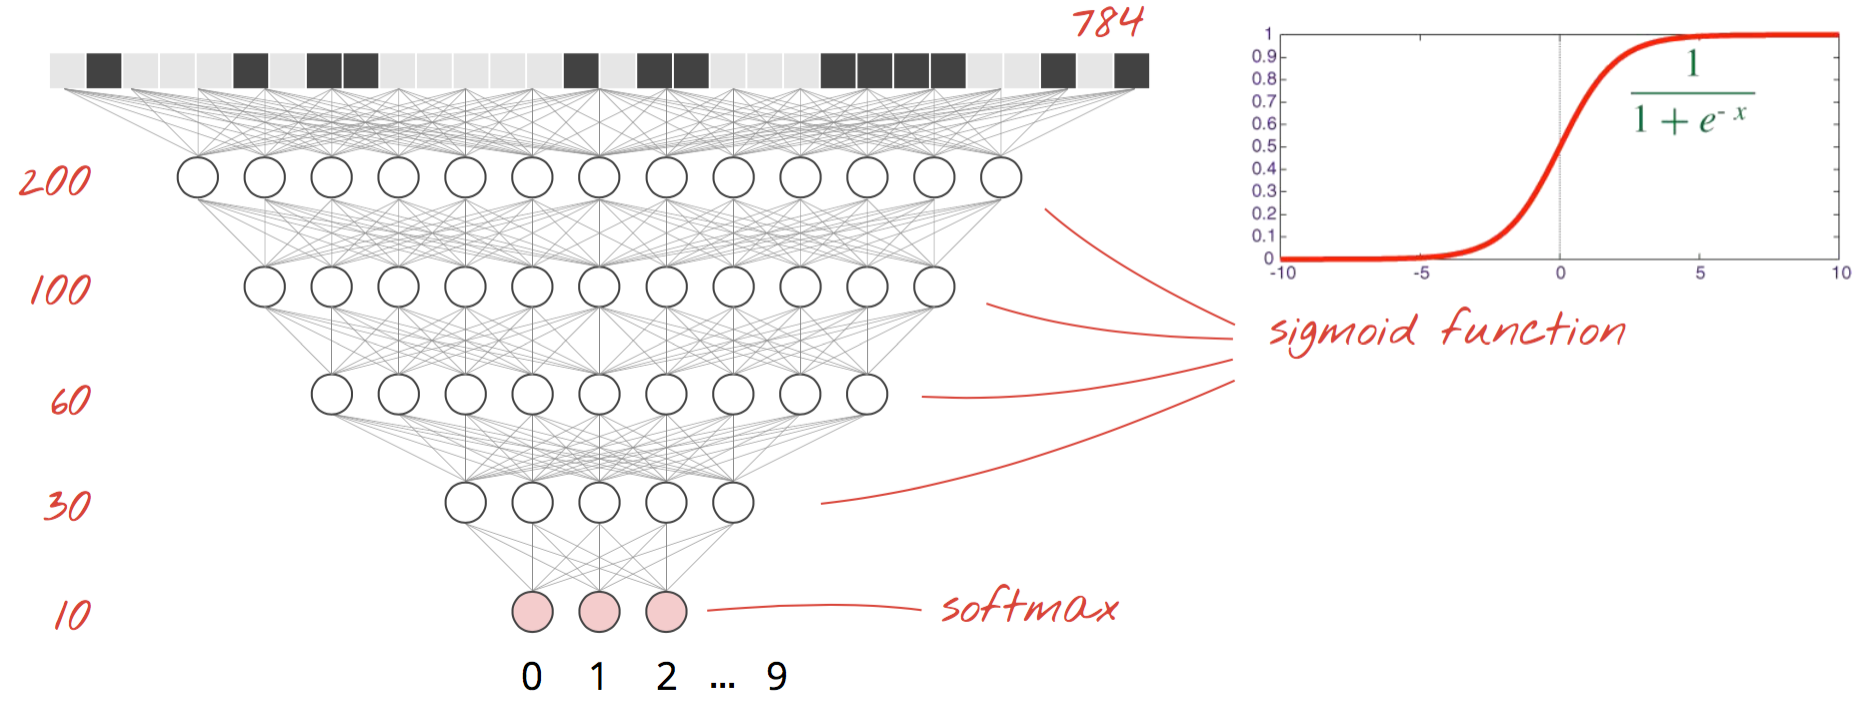
\includegraphics[width=0.8\textwidth]{figures/mnist-5-layer.png}
\caption{5层感知器}
 \label{fig:mnist-5-layer}
\end{figure}

\subsection{理论基础}

\subsubsection{符号定义}

为了形式化地描述多层感知器模型,此处定义了一些常用符号。

\begin{itemize}
   \item \alert{$ {n_{\ell}} $}: 网络层数,其中第$0$层为输入层,第$n_{\ell}$层为输出层
   \item \alert{$ {s_{\ell}} $}: 第$\ell$层的节点数,$ \ell = 0, 1, ..., n_{\ell} $
   \item \alert{$ w_{ji}^{(\ell)} $}: 第$(\ell-1)$层节点$i$与第$\ell$层节点$j$之间的权重,$ \ell = 1, ..., n_{\ell} $
   \item \alert{$ b_i^{(\ell)} $}: 第$\ell$层节点$i$的偏置项,$ \ell = 1, ..., n_{\ell} $
   \item \alert{$ a_i^{(\ell)} $}: 第$\ell$层节点$i$的输出,$ \ell = 1, ..., n_{\ell}, x = a^{(0)}, y = a^{(n_{\ell})} $
   \item \alert{$ z_i^{(\ell)} $}: 第$\ell$层节点$i$的权重和,$ \ell = 1, ..., n_{\ell} $
   \item \alert{$ \delta _i^{(\ell)} $}: 第$\ell$层节点$i$的误差项,$ \ell = 1, ..., n_{\ell} $
   \item \alert{$ S = \{ ({x^{(t)}},{y^{(t)}});t = 1,2,...,m\} $}: 样本空间
 \end{itemize}

\subsubsection{前向传播}

$z^{(\ell )}$表示$\ell$层的线性加权和,它由第$\ell - 1$层的输出$a^{(\ell  - 1)}$与第$\ell$层的权重矩阵$w^{(\ell )}$相乘,再加上第$\ell$层的偏置向量所得。

推而广之,第$\ell$层的输出,由激活函数$f({z^{(\ell )}})$所得。其中,$a^{(0)}} = x, y = {a^{({n_\ell })}}$。

\[\begin{gathered}
  {z^{(\ell )}} = {w^{(\ell )}}{a^{(\ell  - 1)}} + {b^{(\ell )}} \hfill \\
  {a^{(\ell )}} = f({z^{(\ell )}}) \hfill \\
  {a^{(0)}} = x \hfill \\
  y = {a^{({n_\ell })}} \hfill \\ 
\end{gathered} \]

\subsubsection{后向传播}

然后,反向计算各层的误差。其中,第$\ell$层的误差,由$\ell + 1$层的误差计算所得。特殊地,在输出层,预测值$a^{({n_\ell })}$与$y$之间的误差,可以直接计算得到。

\[{\delta ^{(\ell)}} = \left\{ \begin{gathered}
  {({w^{(\ell + 1)}})^T}{\delta ^{(\ell + 1)}} \circ f\,'({z^{(\ell)}});{\text{  }}\ell \ne {n_\ell} \hfill \\
  ({a^{(\ell)}} - y) \circ f\,'({z^{(\ell)}}); {\text{  }}\ell = {n_\ell} \hfill \\ 
\end{gathered}  \right.\]

损失函数$J(w,b)$相对于各层的权重矩阵与偏置向量的梯度便可以计算得到。

\[\begin{gathered}
  {\nabla _{{w^{(\ell )}}}}J(w,b;x,y) = {\delta ^{(\ell )}}{\left( {{a^{(\ell  - 1)}}} \right)^T} \hfill \\
  {\nabla _{{b^{(\ell )}}}}J(w,b;x,y) = {\delta ^{(\ell )}} \hfill \\
  \ell  = 1,2,...,{n_\ell } \hfill \\ 
\end{gathered} \]

一般地,在实际系统实现中,下游层传递梯度给上层,上层直接完成梯度的计算。

\subsubsection{参数更新}

对于给定样本数据集$ S = \{ ({x^{(t)}},{y^{(t)}});t = 1,2,...,m\} $,根据梯度反传公式,可以计算得到参数更新的变化量。

\[\begin{aligned}
  \Delta {w^{(\ell )}} \leftarrow \Delta {w^{(\ell )}} + {\nabla _{{w^{(\ell )}}}}J\left( {w,b;{x^{(t)}},{y^{(t)}}} \right) \\ 
  \Delta {b^{(\ell )}} \leftarrow \Delta {b^{(\ell )}} + {\nabla _{{b^{(\ell )}}}}J\left( {w,b;{x^{(t)}},{y^{(t)}}} \right) \\ 
  t = 1,2,...,m;\ell  = 1,2,...,{n_\ell } \\ 
\end{aligned} \]

最后,执行梯度下降算法,完成训练参数一个迭代的更新。

\[\begin{aligned}
  {w^{(\ell )}} \leftarrow  & {w^{(\ell )}} - \alpha \left( {\frac{{\Delta {w^{(\ell )}}}}{m}} \right) \\ 
  {b^{(\ell )}} \leftarrow  & {b^{(\ell )}} - \alpha \frac{{\Delta {b^{(\ell )}}}}{m} \\ 
  \ell  = & 1,2,...,{n_\ell }  \\
\end{aligned} \]

\subsection{定义模型}

相对于上一节中尝试的单层感知器,此处定义每一个隐式层的权重时,并没有使用常量定义变量的初始值,而使用满足某种数据分布特征的随机值。

\begin{leftbar}
\begin{python}
K = 200
L = 100
M = 60
N = 30

w1 = tf.Variable(tf.truncated_normal([28*28, K] ,stddev=0.1)) 
b1 = tf.Variable(tf.zeros([K]))

w2 = tf.Variable(tf.truncated_normal([K, L], stddev=0.1))
b2 = tf.Variable(tf.zeros([L]))

w3 = tf.Variable(tf.truncated_normal([L, M], stddev=0.1)) 
b3 = tf.Variable(tf.zeros([M]))

w4 = tf.Variable(tf.truncated_normal([M, N], stddev=0.1)) 
b4 = tf.Variable(tf.zeros([N]))

w5 = tf.Variable(tf.truncated_normal([N, 10], stddev=0.1)) 
b5 = tf.Variable(tf.zeros([10]))
\end{python}
\end{leftbar}

在定义每一个隐式层时,采用\ascii{sigmoid}的激活函数。而在最后的输出层,采用\ascii{softmax}的激活函数。

\begin{leftbar}
\begin{python}
y1 = tf.nn.sigmoid(tf.matmul(x,  w1) + b1)
y2 = tf.nn.sigmoid(tf.matmul(y1, w2) + b2)
y3 = tf.nn.sigmoid(tf.matmul(y2, w3) + b3)
y4 = tf.nn.sigmoid(tf.matmul(y3, w4) + b4)
y  = tf.nn.softmax(tf.matmul(y4, w5) + b5)
\end{python}
\end{leftbar}

经过迭代的模型训练,可以得到大约\percent{97}左右的精度。但是,网络随着层次的增加,模型变得越来越难以收敛。接下来,尝试一些常见的调优技术,改善网络的性能。

\subsection{优化技术}

\subsubsection{激活函数:ReLU}

在深度模型中,不适合使用\ascii{sigmoid}激活函数。它将把所有的值都挤到了\ascii{0}到\ascii{1}之间;随着网络层次的增加,引发梯度消失的问题。

\begin{figure}[H]
\centering
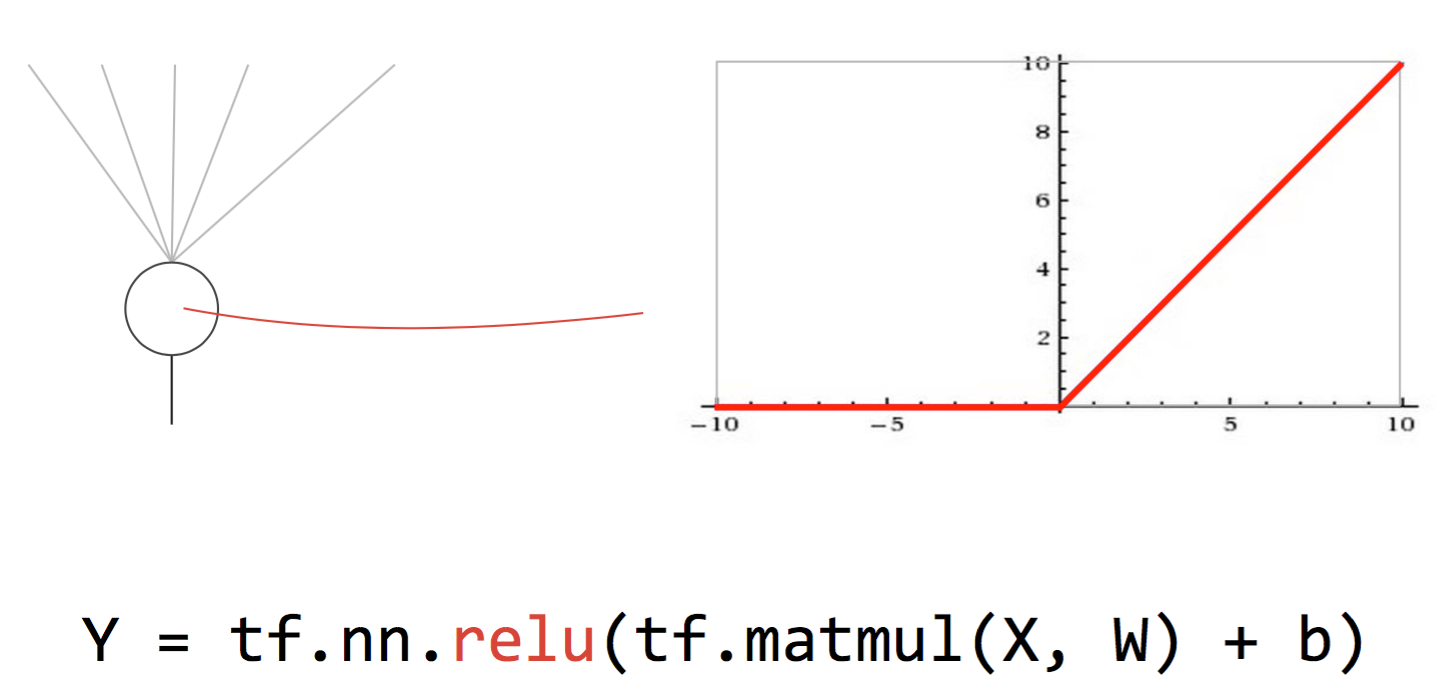
\includegraphics[width=0.8\textwidth]{figures/mnist-relu.png}
\caption{ReLU激活函数}
 \label{fig:mnist-relu}
\end{figure}

可以使用\ascii{ReLU(Rectified Linear Unit)}替代\ascii{sigmoid},不仅避免了\ascii{sigmoid}导致的一些问题,而且能够加快初始的收敛速度。

\begin{leftbar}
\begin{python}
y1 = tf.nn.relu(tf.matmul(x,  w1) + b1)
y2 = tf.nn.relu(tf.matmul(y1, w2) + b2)
y3 = tf.nn.relu(tf.matmul(y2, w3) + b3)
y4 = tf.nn.relu(tf.matmul(y3, w4) + b4)
y  = tf.nn.softmax(tf.matmul(y4, w5) + b5)
\end{python}
\end{leftbar}

另外,如果使用\ascii{ReLU}激活函数,偏置向量常常初始化为小的正值,使得神经元在一开始就会工作在\ascii{ReLU}的非零区域内。

\begin{leftbar}
\begin{python}
K = 200
L = 100
M = 60
N = 30

w1 = tf.Variable(tf.truncated_normal([28*28, K] ,stddev=0.1)) 
b1 = tf.Variable(tf.ones([L])/10)

w2 = tf.Variable(tf.truncated_normal([K, L], stddev=0.1))
b2 = tf.Variable(tf.ones([L])/10)

w3 = tf.Variable(tf.truncated_normal([L, M], stddev=0.1)) 
b3 = tf.Variable(tf.ones([L])/10)

w4 = tf.Variable(tf.truncated_normal([M, N], stddev=0.1)) 
b4 = tf.Variable(tf.ones([L])/10)

w5 = tf.Variable(tf.truncated_normal([N, 10], stddev=0.1)) 
b5 = tf.Variable(tf.ones([L])/10)
\end{python}
\end{leftbar}

如\refig{mnist-sigmoid-to-relu}所示,前\ascii{300}次迭代,使用\ascii{ReLU}相对于使用\ascii{sigmoid},其初始收敛速度提升显著。

\begin{figure}[H]
\centering
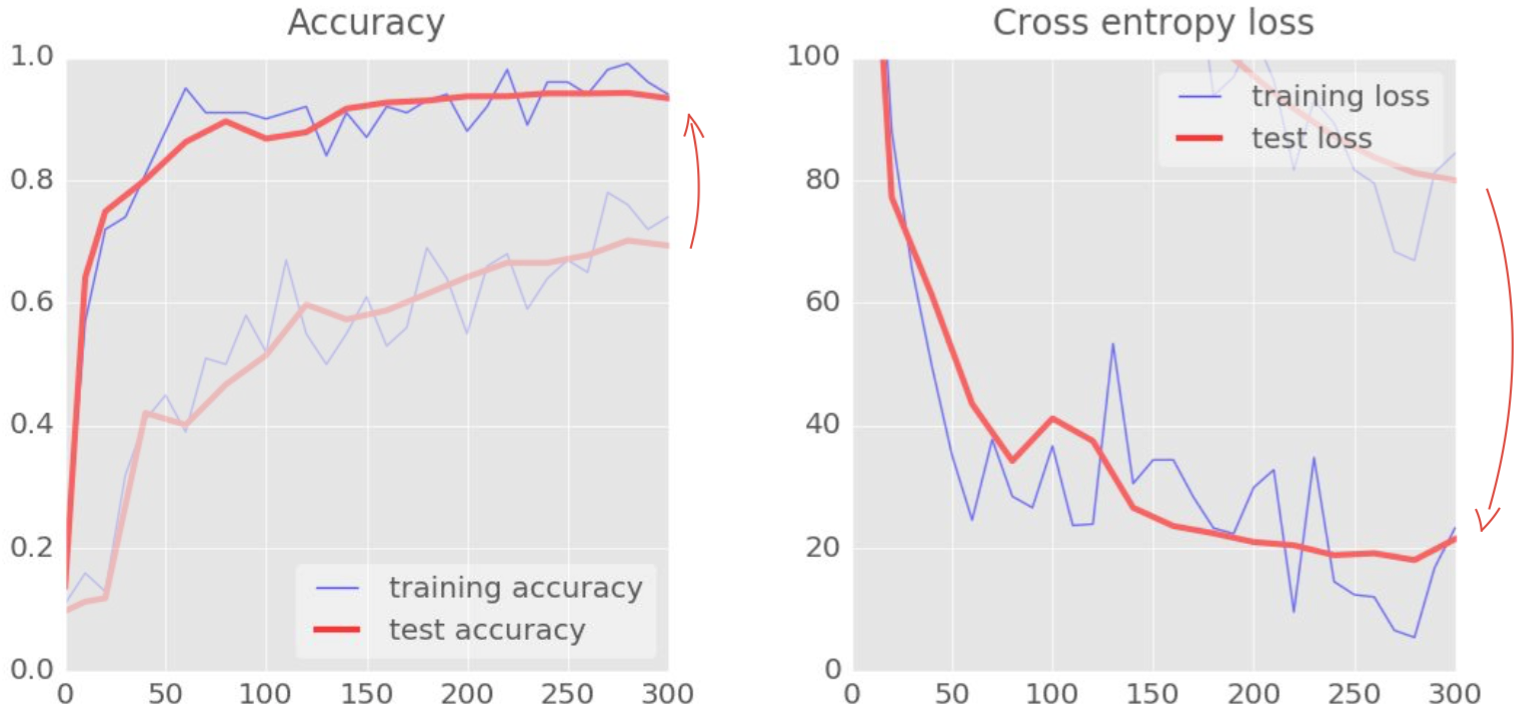
\includegraphics[width=0.8\textwidth]{figures/mnist-sigmoid-to-relu.png}
\caption{应用ReLU激活函数:初始收敛速度提升显著}
 \label{fig:mnist-sigmoid-to-relu}
\end{figure}

\subsubsection{不定值}

为了得到稳定的数值计算结果,避免出现精度突降为\ascii{0}的情况发生。追溯实现代码,可能引入\code{log(0)}计算得到\code{NaN}不定值的问题。可以使用\code{softmax\_cross\_entropy\_with\_logits}计算交叉熵损失,并将线性加权和作为其输入(常称为\ascii{logits})。

\begin{leftbar}
\begin{python}
logits = tf.matmul(y4, w5) + b5
y = tf.nn.softmax(logits)

cross_entropy = tf.nn.softmax_cross_entropy_with_logits(
  logits=logits, labels=t)
\end{python}
\end{leftbar}

\subsubsection{学习速率衰减}

随着网路层次的增加,及其应用相关优化技术后,模型的精度能够能得到\percent{98}左右,但很难得到一个稳定的精度。如\refig{mnist-lr-too-larger}所示,精度和损失抖动相当明显。

\begin{figure}[H]
\centering
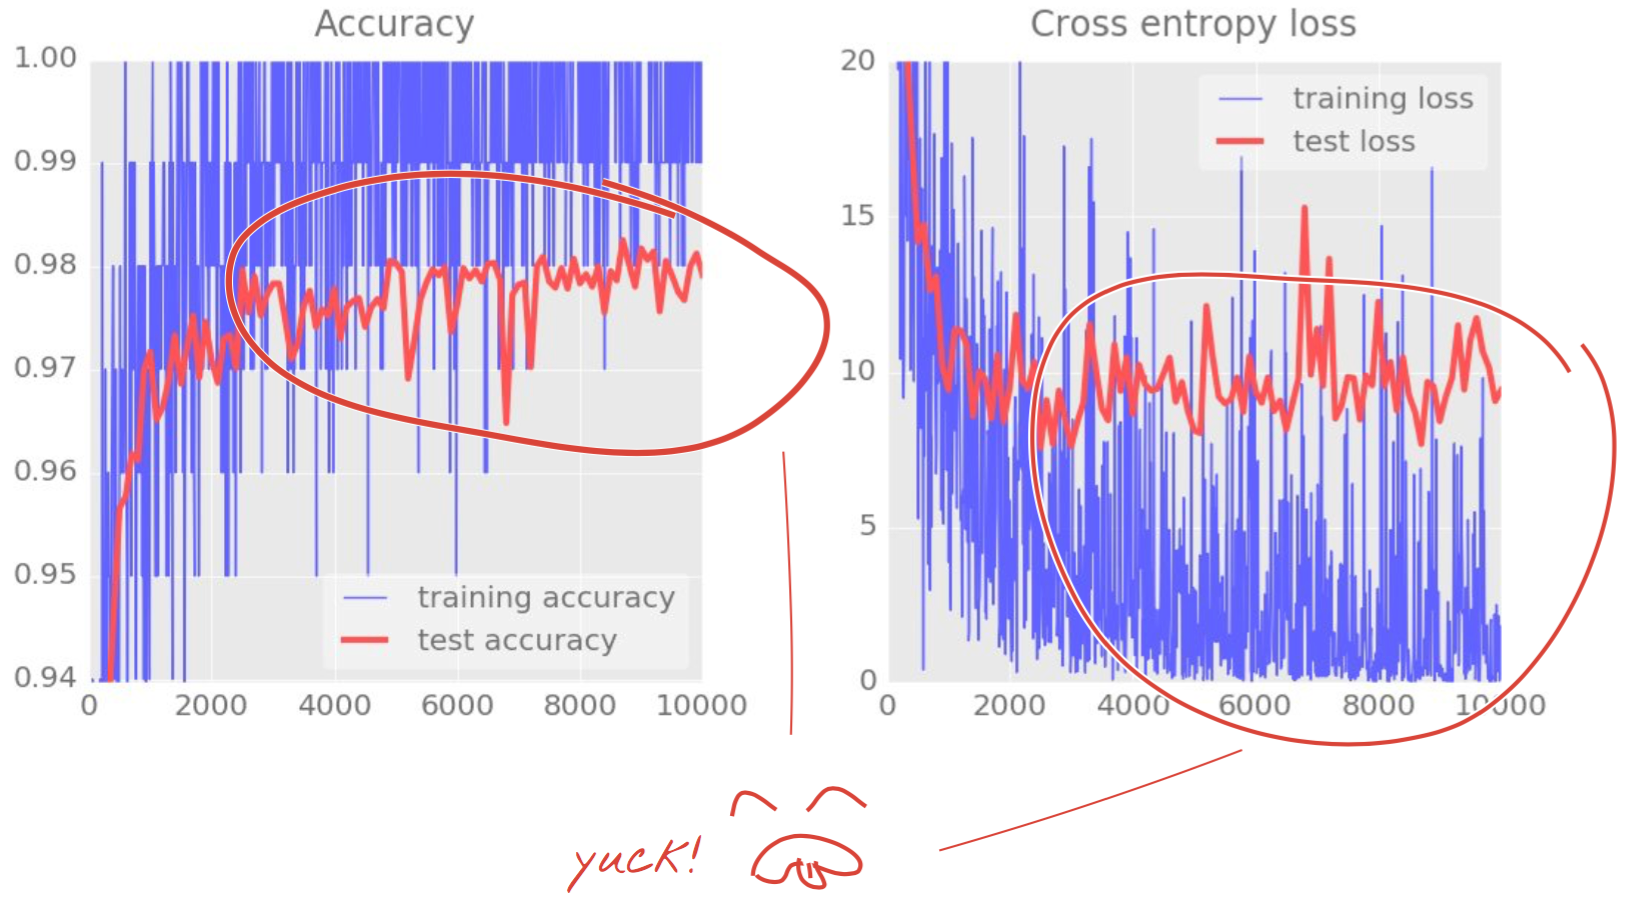
\includegraphics[width=0.8\textwidth]{figures/mnist-lr-too-larger.png}
\caption{噪声抖动:学习速率过大}
 \label{fig:mnist-lr-too-larger}
\end{figure}

可以采用更好的优化算法,例如\code{AdamOptimizer}。随着迭代过程的次数,学习速率将指数级衰减,在模型训练后期可以得到一个更稳定的精度和损失曲线。

\begin{leftbar}
\begin{python}
lr = tf.placeholder(tf.float32)
train_step = tf.train.AdamOptimizer(lr).minimize(cross_entropy)
\end{python}
\end{leftbar}

在每个迭代训练过程中,根据当前\code{step}的值,实时计算当前迭代的学习速率\code{lr},然后通过\code{feed\_dict}传递给\code{Session.run}执行。其中,学习速率衰减方程如下代码所示,随着迭代次数的增加,学习速率指数衰减。

\begin{leftbar}
\begin{python}
def lr(step):
  max_lr, min_lr, decay_speed = 0.003, 0.0001, 2000.0
  return min_lr + (max_lr - min_lr) * math.exp(-step/decay_speed)

with tf.Session() as sess:
  for step in range(10000):
    batch_xs, batch_ys = mnist.train.next_batch(100)
    sess.run(train_step, 
      feed_dict={x: batch_xs, t: batch_ys, pkeep: 0.75, lr: lr(step)})
\end{python}
\end{leftbar}

如\refig{mnist-apply-learning-rate-decay}所示,应用学习速率衰减方法后,可以得到一个更稳定的精度和损失曲线。

\begin{figure}[H]
\centering
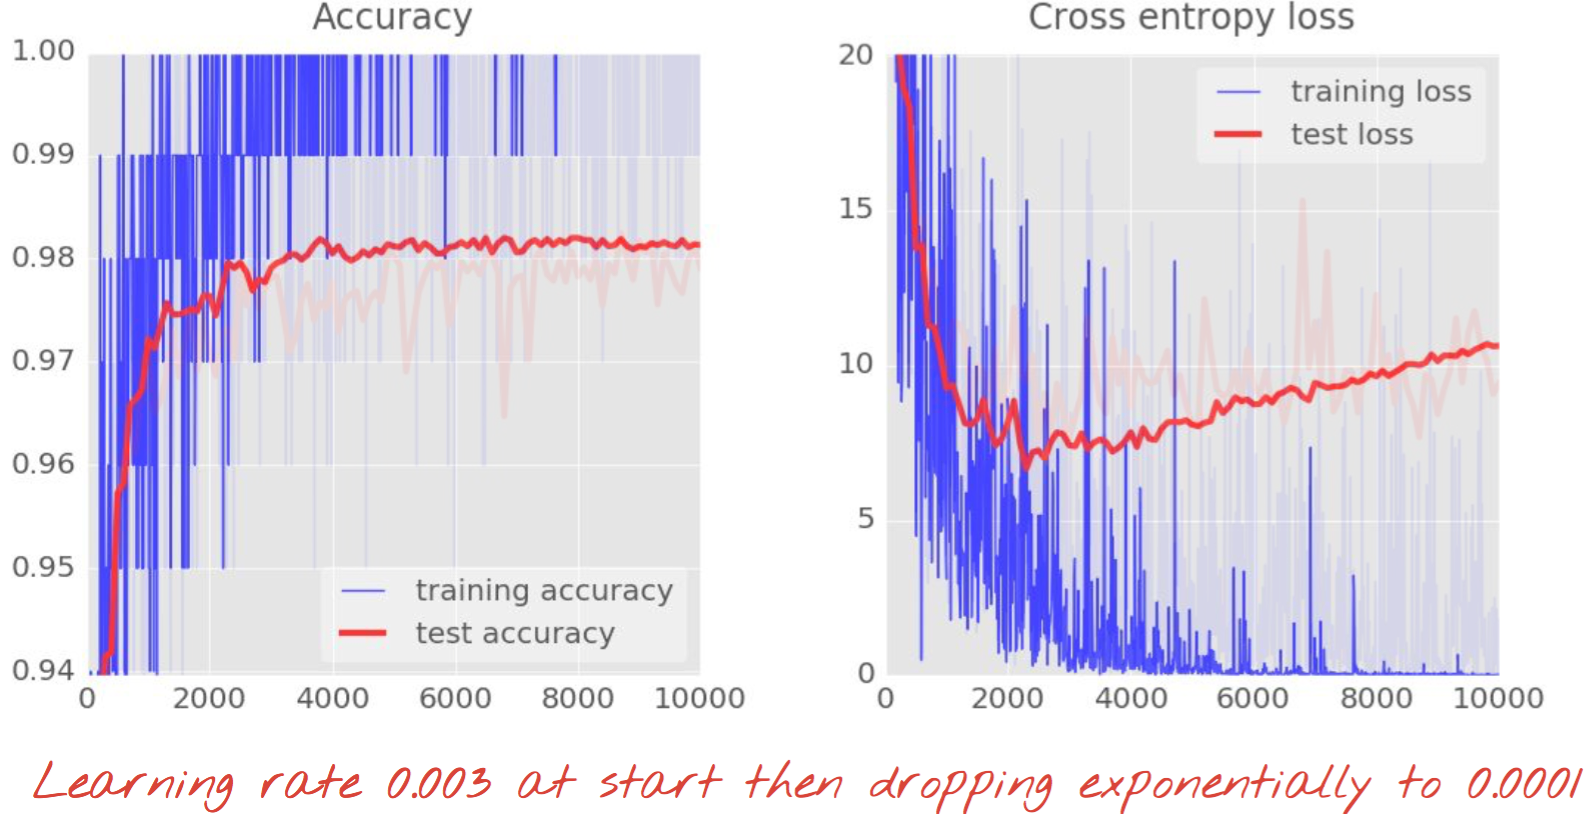
\includegraphics[width=0.8\textwidth]{figures/mnist-apply-learning-rate-decay.png}
\caption{应用Adam优化算法后,精度和损失趋于稳定}
 \label{fig:mnist-apply-learning-rate-decay}
\end{figure}

\subsubsection{应用Dropout}

但是,损失曲线在训练集与测试集上相分离,出现明显的过拟合现象。即模型在训练数据集上表现良好,但在测试数据集上出现反弹,模型缺乏足够的泛化能力。

\begin{figure}[H]
\centering
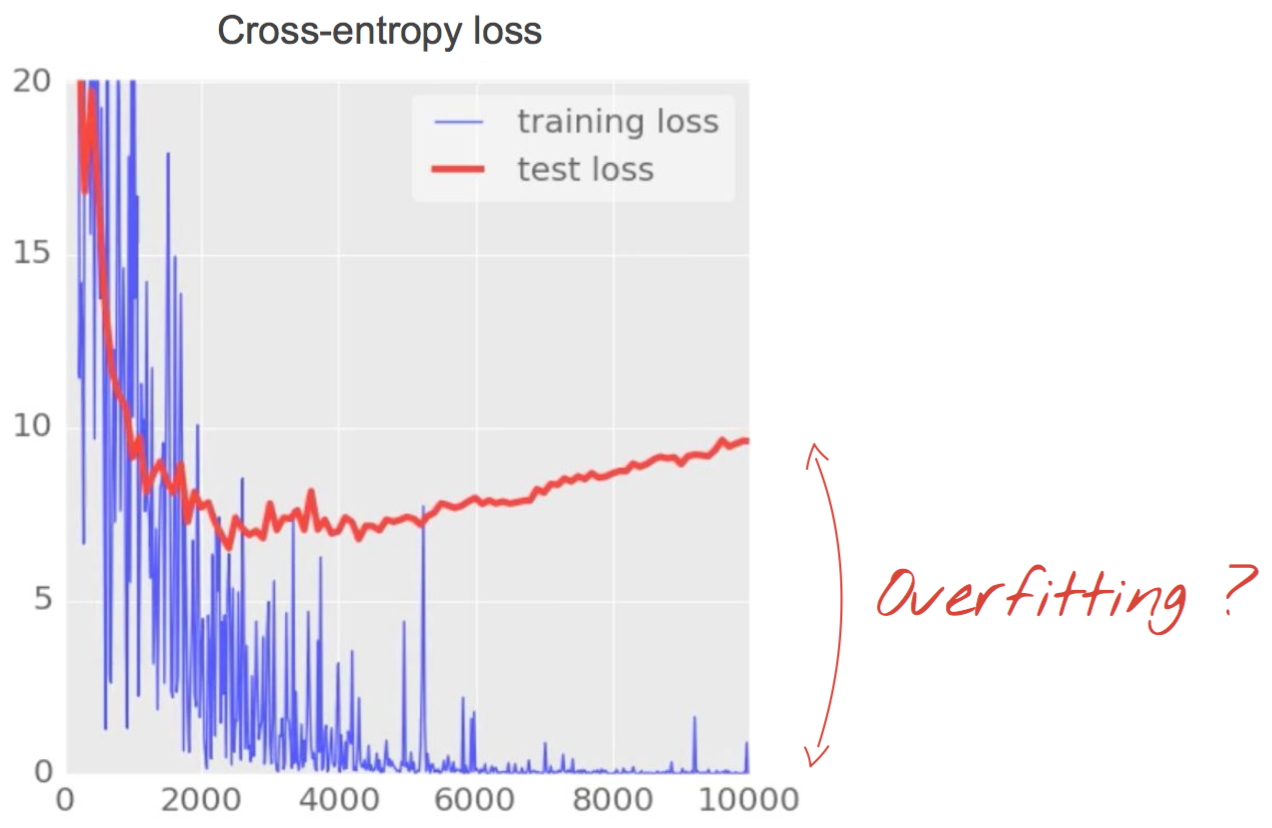
\includegraphics[width=0.8\textwidth]{figures/mnist-overfitting.png}
\caption{过拟合}
 \label{fig:mnist-overfitting}
\end{figure}

如\refig{mnist-dropout}所示,在训练时对隐藏层的输出实施\ascii{dropout}操作,以\code{1 - pkeep}的概率随机丢弃神经元的输出,并在反向传播梯度时不再更新相应的权重。而在推理时恢复所有神经元的输出,间接改善了网络的泛化能力。

\begin{figure}[H]
\centering
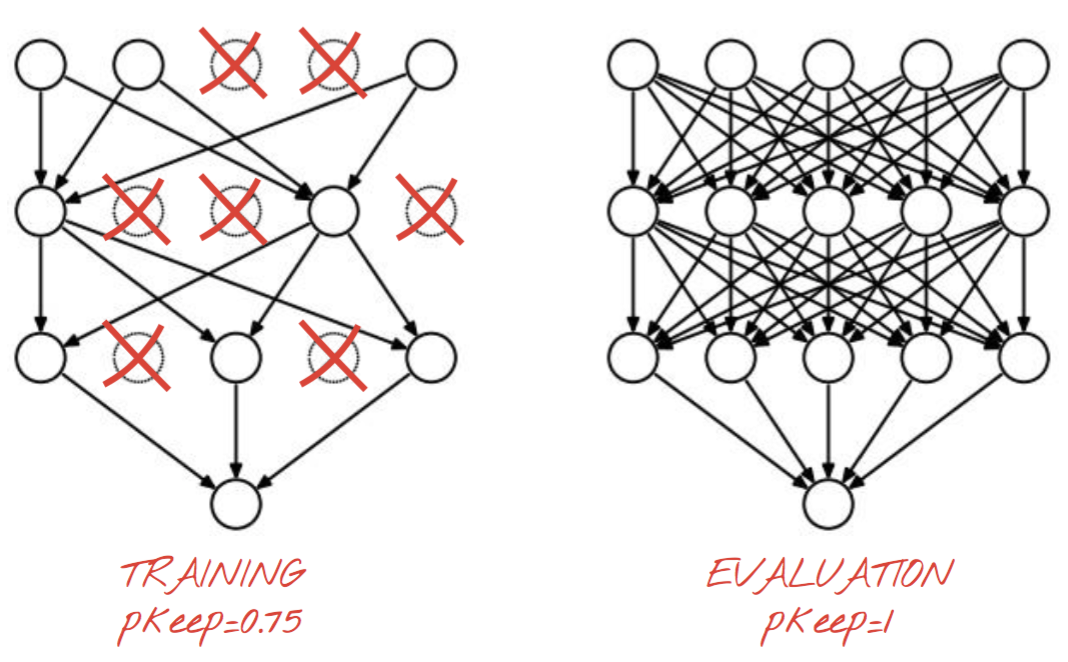
\includegraphics[width=0.8\textwidth]{figures/mnist-dropout.png}
\caption{Dropout方法}
 \label{fig:mnist-dropout}
\end{figure}

使用\tf{}实现\ascii{dropout}操作时,先定义一个超级参数\code{pkeep},表示隐藏层的神经元以概率\code{pkeep}随机保留,以概率\code{1 - pkeep}随机丢弃。

\begin{leftbar}
\begin{python}
pkeep = tf.placeholder(tf.float32)

y1 = tf.nn.relu(tf.matmul(x,  w1) + b1)
y1d = tf.nn.dropout(y1, pkeep)

y2 = tf.nn.relu(tf.matmul(y1d, w2) + b2)
y2d = tf.nn.dropout(y2, pkeep)

y3 = tf.nn.relu(tf.matmul(y2d, w3) + b3)
y3d = tf.nn.dropout(y3, pkeep)

y4 = tf.nn.relu(tf.matmul(y3d, w4) + b4)
y4d = tf.nn.dropout(y4, pkeep)

logits = tf.matmul(y4d, w5) + b5
y = tf.nn.softmax(Ylogits)
\end{python}
\end{leftbar}

在训练时,置超参\code{pkeep}的值小于\ascii{1};而在推理时,置超参\code{pkeep}的值为\ascii{1}。

\begin{leftbar}
\begin{python}
with tf.Session() as sess:
  for step in range(10000):
    batch_xs, batch_ys = mnist.train.next_batch(100)
    sess.run(train_step, 
      feed_dict={x: batch_xs, t: batch_ys, pkeep: 0.75, lr: lr(step)})

    if step % 100 == 0:
      acc, loss = sess.run([accuracy, cross_entropy], 
        feed_dict={x: batch_xs, t: batch_ys, pkeep: 1})
      acc, loss = sess.run([accuracy, cross_entropy], 
        feed_dict={x: mnist.test.images, t: mnist.test.labels, pkeep: 1})
\end{python}
\end{leftbar}

在每一隐藏层实施\ascii{dropout}操作之后,训练集与测试集的损失曲线再次相交。但是,精度和损失曲线相比又出现小幅的抖动,而且训练集与测试集的损失曲线相重合的程度不是很理想,过拟合问题依然很突出。

也就是说,过拟合问题存在其他更深刻的原因。例如,将$ 28 \times 28 $的图片实施扁平化操作,将其变换为一个长度为\ascii{784}的一维向量,这将完全丢失了像素的空间排列信息。

接下来,通过尝试构造卷积神经网络,从原图像中提取特征,从而保留了像素的空间排列信息,进而提升网络的性能。

\begin{figure}[H]
\centering
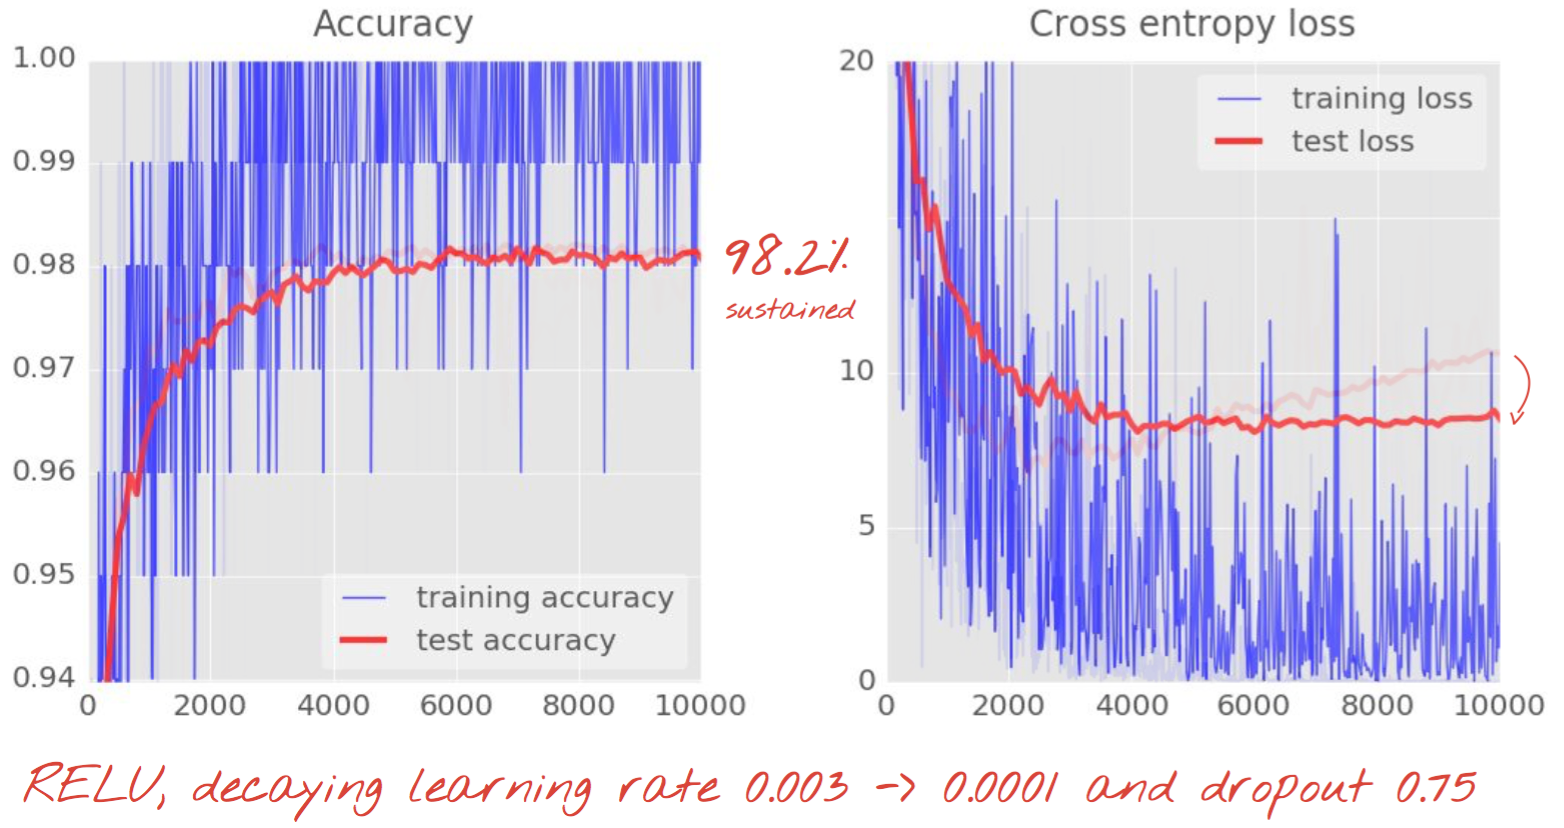
\includegraphics[width=0.8\textwidth]{figures/mnist-apply-dropout-result.png}
\caption{实施Dropout后,训练集与测试集的损失曲线再次重合}
 \label{fig:mnist-apply-dropout-result}
\end{figure}

\end{content}

\section{卷积网络}

\begin{content}

\subsection{特征与优势}

随着网络层次增加,全连接网络的梯度消失的问题将越发突出,收敛速度变得越来越慢。相对于全连接网络,卷积网络具有\ascii{3}个主要特征,它减少了网络参数的数量,提升网络的泛化能力。

\subsubsection{局部连接}

相对于全连接网络,卷积网络实现了局部连接,即每个神经元并不与上一层的神经元都存在连接。如\refig{mnist-conv-local-conn}左侧所示,假如存在一张$ 1000 \times 1000 $像素的图像,及其$ 10^6 $个隐藏层的神经元。在全连接网络里,将拥有$ 10^3 \times 10^3 \times 10^6 = 10^{12} $个训练参数。

事实上,每个神经元没有必要与上一层神经元都存在连接。如\refig{mnist-conv-local-conn}右侧所示,假如每个隐藏层的神经元仅与上一层$ 10 \times 10 $的局部图像存在连接,$ 10^6 $个隐藏层的神经元则需要$ 10^6 \times 10^2 = 10^8$个网络连接,相比减少了\ascii{4}个数量级。

\begin{figure}[H]
\centering
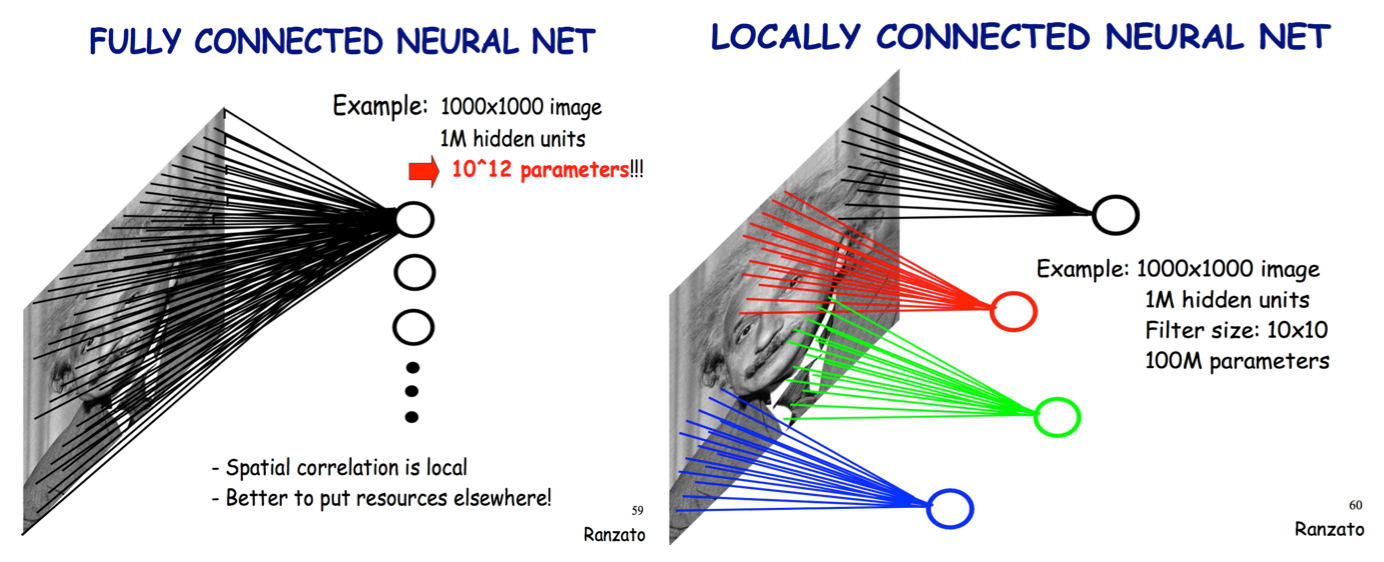
\includegraphics[width=0.9\textwidth]{figures/mnist-conv-local-conn.png}
\caption{局部连接}
 \label{fig:mnist-conv-local-conn}
\end{figure}

\subsubsection{权值共享}

为了进一步减少网络连接,卷积网络还实现了权重共享;即每一组连接共享相同的权重,而不是每个连接存在不同的权重。如\refig{mnist-conv-local-conn-2}右侧所示,每个隐藏层的神经元仅与$ 10 \times 10 $的局部图像存在连接,且共享$ 10 \times 10 $的权重矩阵,与隐藏层的神经元的数目无关。相对于如\refig{mnist-conv-local-conn-2}左侧的局部连接网络,需要$10^8$个参数,卷积层仅需$10^2$个参数。

如\refig{mnist-conv-local-conn-2}右侧所示,为了提取不同特征,例如不同边缘的图像特征,可以使用多个过滤器。例如,存在\ascii{100}个过滤器,则需要$10^4$个参数。

\begin{figure}[H]
\centering
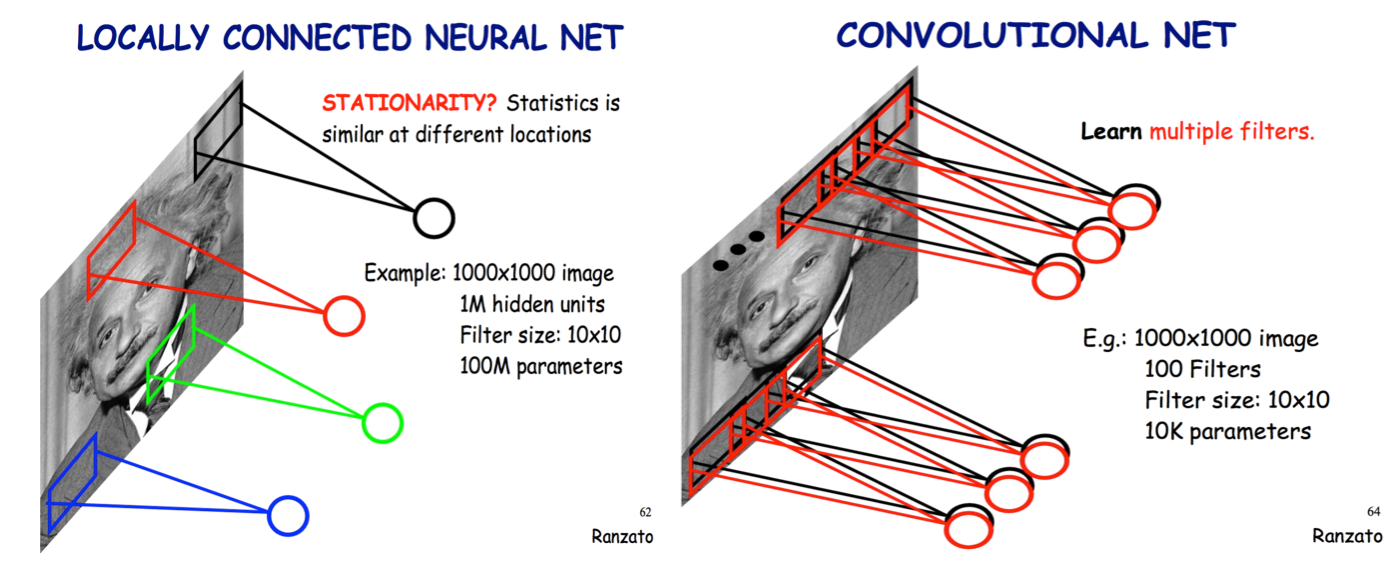
\includegraphics[width=0.9\textwidth]{figures/mnist-conv-local-conn-2.png}
\caption{权值共享,多个过滤器}
 \label{fig:mnist-conv-local-conn-2}
\end{figure}

\subsubsection{下采样}

如\refig{mnist-subsample}所示,可选地实施下采样,进一步减少网络的参数,提升模型的鲁棒性。

\begin{figure}[H]
\centering
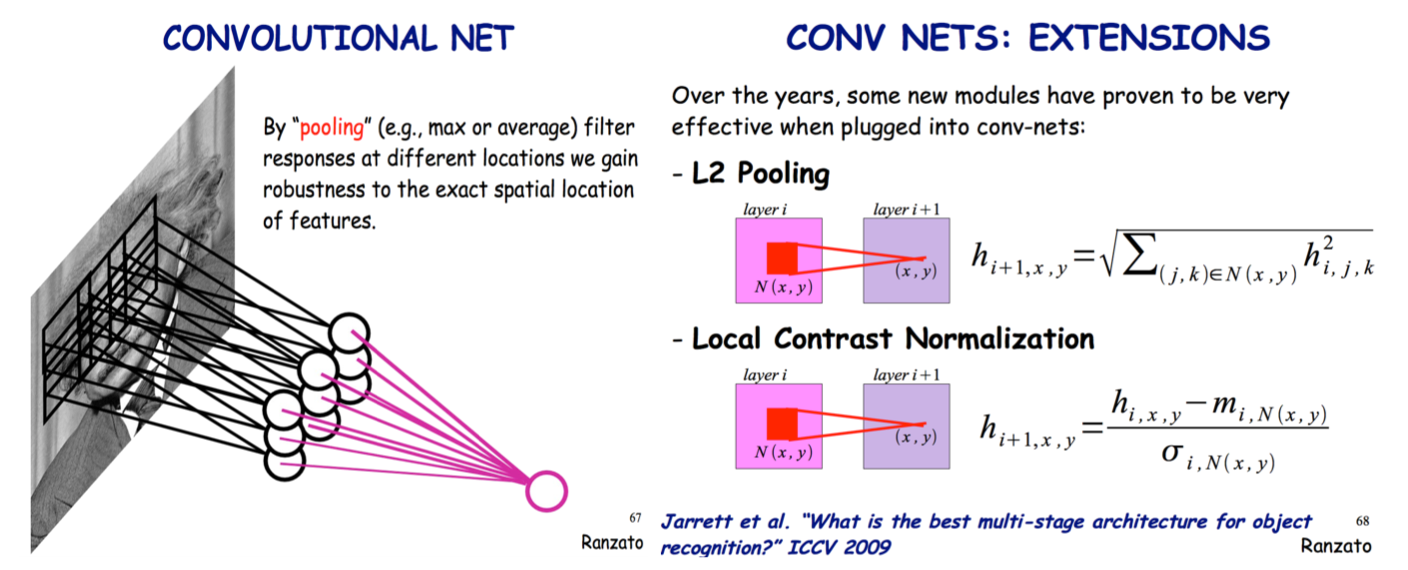
\includegraphics[width=0.9\textwidth]{figures/mnist-subsample.png}
\caption{下采样}
 \label{fig:mnist-subsample}
\end{figure}

\subsection{卷积运算}

卷积运算是一个计算密集型的\ascii{OP}。如\refig{mnist-conv2d-gif}所示,存在一个权重向量\code{w[3,3,3,2]},其中输入通道数为\ascii{3},输出通道数为\ascii{2},卷积核大小为$3 \times 3$。

显而易见,输入图像的通道数,等价于卷积核的深度;卷积核的数目,等于\ascii{Feature Map}的输出通道数。另外,为了采集图像的边缘特征,在原图像外围补了(\ascii{padding})一圈零值。每次卷积计算,移动的步长(\ascii{stride})为\ascii{2}。因此,最终输出的\ascii{Feature Map}大小为$3 \times 3$。

\begin{figure}[H]
\centering
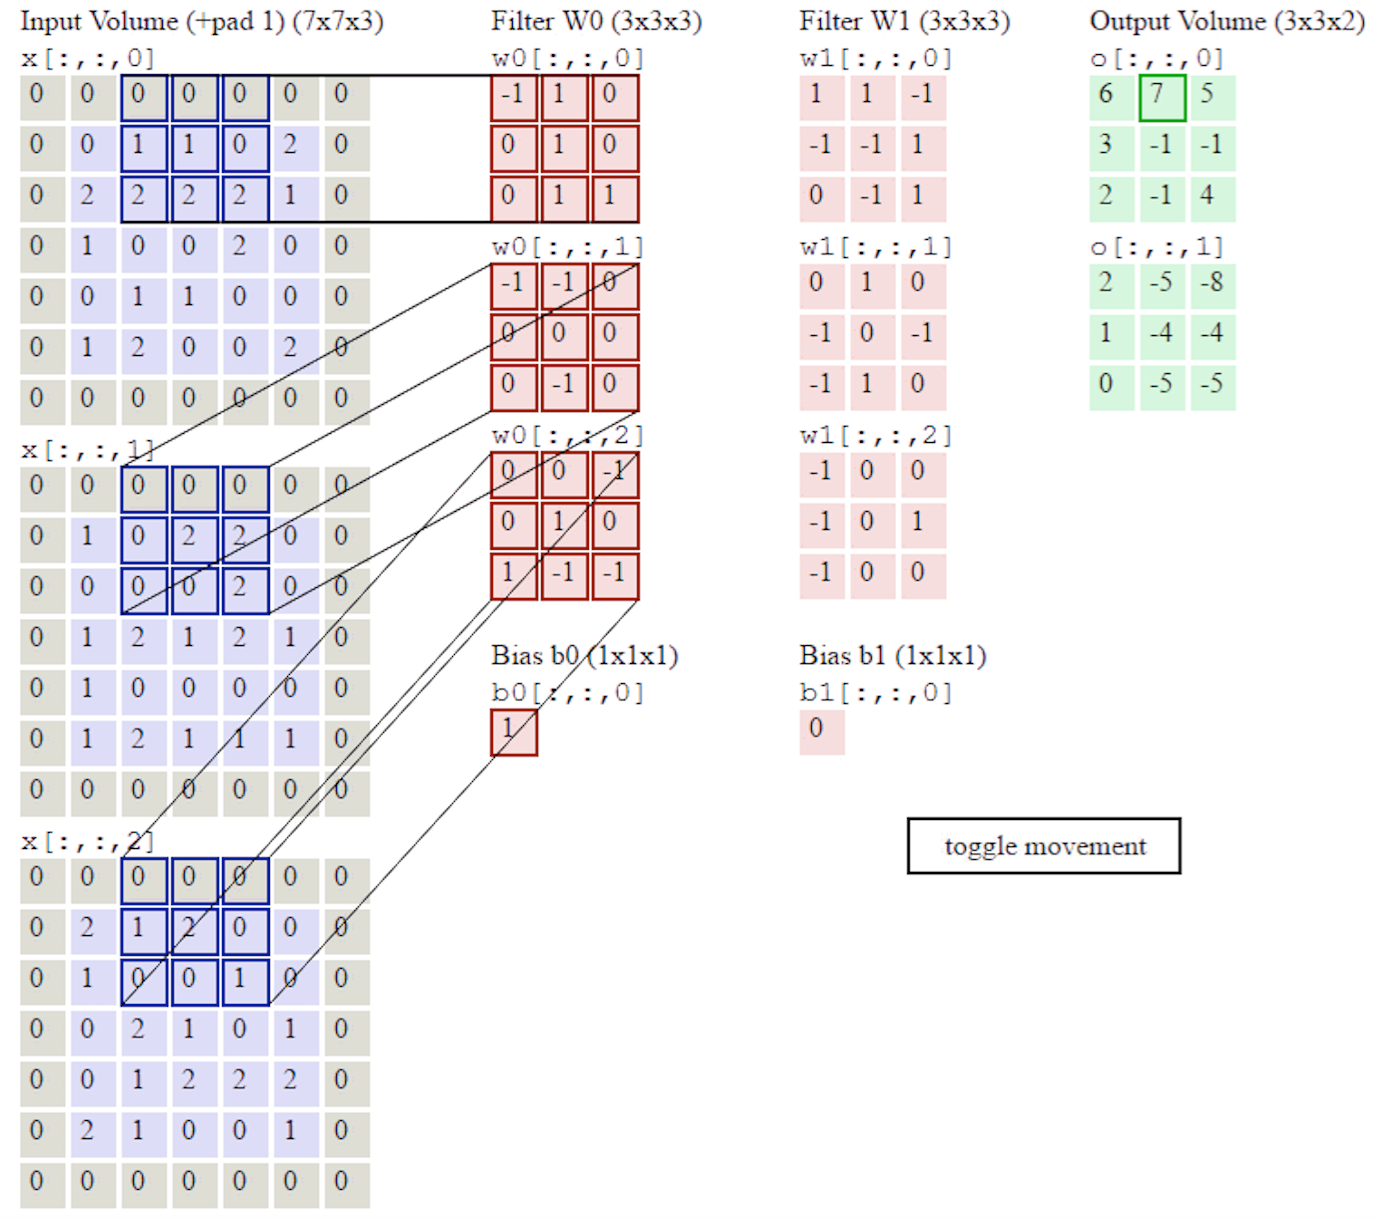
\includegraphics[width=0.8\textwidth]{figures/mnist-conv2d-gif.png}
\caption{卷积运算}
 \label{fig:mnist-conv2d-gif}
\end{figure}

\subsubsection{例子}

假如存在一个$32 \times 32 \times 3$的图片,卷积核大小为$5 \times 5 \times 3$。其中,卷积核的深度等于图片的输入通道数。如\refig{mnist-conv-1dot}所示,卷积核与图片中大小为$5 \times 5 \times 3$的块实施点积运算,得到一个值。

\begin{figure}[H]
\centering
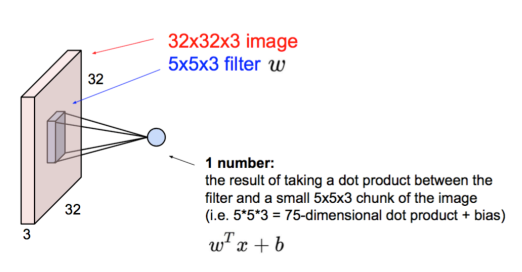
\includegraphics[width=0.8\textwidth]{figures/convolutional-layer-2.png}
\caption{卷积运算:卷积核与图片块的点积运算}
 \label{fig:mnist-conv-1dot}
\end{figure}

如\refig{mnist-conv-ndot}所示,卷积核遍历整个图片空间,最终得到一个大小为$28 \times 28 \times 1$的\ascii{Feature Map}。

\begin{figure}[H]
\centering
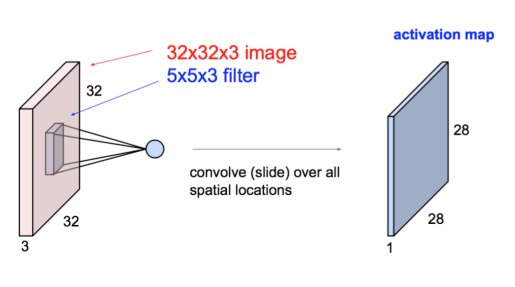
\includegraphics[width=0.8\textwidth]{figures/convolutional-layer-3.png}
\caption{卷积运算:卷积核遍历图片,步长为1}
 \label{fig:mnist-conv-ndot}
\end{figure}

如\refig{mnist-conv-multi-filters}所示,如果存在多个卷积核,则得到多个\ascii{Feature Map}。

\begin{figure}[H]
\centering
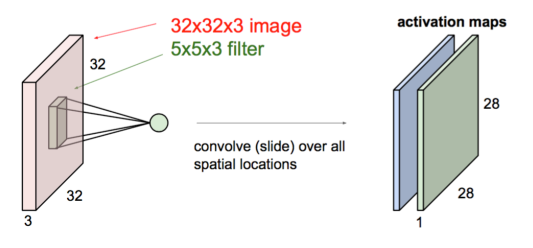
\includegraphics[width=0.8\textwidth]{figures/convolutional-layer-4.png}
\caption{卷积运算:多个卷积核}
 \label{fig:mnist-conv-multi-filters}
\end{figure}

\subsection{公式推导}

\subsubsection{前向传播}

$Z^{(\ell )}$表示$\ell$层的线性加权和,它由第$\ell - 1$层的输出$A^{(\ell  - 1)}$与第$\ell$层的权重矩阵$W^{(\ell )}$卷积,再加上第$\ell$层的偏置向量所得。

推而广之,第$\ell$层的输出,由激活函数$f({Z^{(\ell )}})$所得。其中,$A^{(0)}} = x, y = {A^{({n_\ell })}}$。

\[\begin{gathered}
  {Z^{(\ell )}} = {A^{(\ell  - 1)}} * {W^{(\ell )}} + {b^{(\ell )}} \hfill \\
  {A^{(\ell )}} = f\left( {{Z^{(\ell )}}} \right) \hfill \\ 
\end{gathered} \]

\subsubsection{后向传播}

然后,反向计算各层的误差。其中,第$\ell$层的误差,由$\ell + 1$层的误差计算所得。相对于全连接网络,此处运用的是卷积运算,并非矩阵乘法运算。

\[
{\delta ^{(\ell )}} = {\delta ^{(\ell  + 1)}} * {W^{(\ell  + 1)}} \circ f\,'\left( {{z^{(\ell )}}} \right)
\]

损失函数$J(w,b)$相对于各层的权重矩阵与偏置向量的梯度便可以计算得到。

\[\begin{aligned}
  {\nabla _{{W^{(\ell )}}}}J(W,b) =  & {A^{(\ell  - 1)}} * {\delta ^{(\ell )}} \\ 
  {\nabla _{{b^{(\ell )}}}}J(W,b) =  & {\delta ^{(\ell )}} \\ 
\end{aligned} \]

\subsection{实现卷积网络}

实现卷积网络时,首先需要定义每层过滤器的权重矩阵,用于提取图像的特征。权重矩阵在图像里表现的像一个从原始图像矩阵中提取特定信息的过滤器。一个权重矩阵可能用来提取图像边缘信息,一个权重矩阵可能是用来提取一个特定颜色,另一个权重矩阵可能对不需要的噪声进行模糊化。

当存在多个卷积层时,初始层往往提取较多的一般特征;随着网络结构变得更深,权值矩阵提取的特征越来越复杂,并且越来越适用于眼前的具体问题。

一般地,过滤器常使用一个\ascii{4}维的张量表示,前两维表示过滤器的大小,第三维表示输入的通道数,第四维表示输出的通道数。如\refig{mnist-filter}所示。

\begin{figure}[H]
\centering
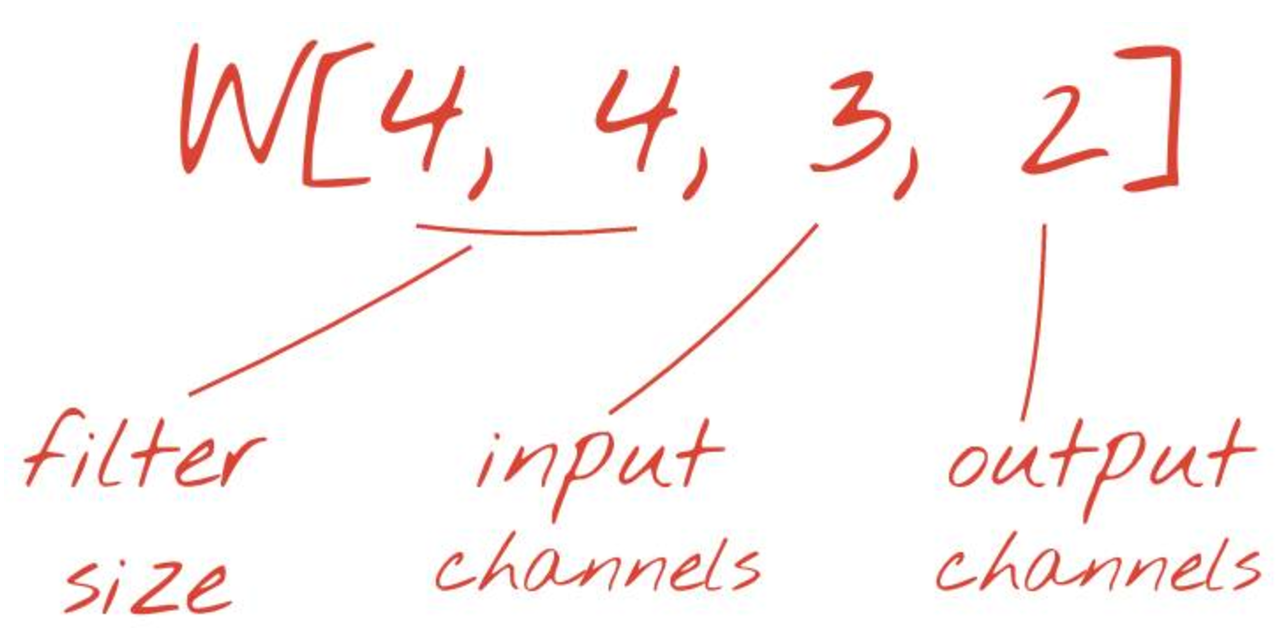
\includegraphics[width=0.4\textwidth]{figures/mnist-filter.png}
\caption{卷积层的过滤器}
 \label{fig:mnist-filter}
\end{figure}

如\refig{mnist-conv2d-1}所示,构造了\ascii{3}个卷积层和\ascii{2}个全连接层。其中,中间隐藏层使用\ascii{ReLU}的激活函数,最后的输出层采用\ascii{softmax}的激活函数。

\begin{figure}[H]
\centering
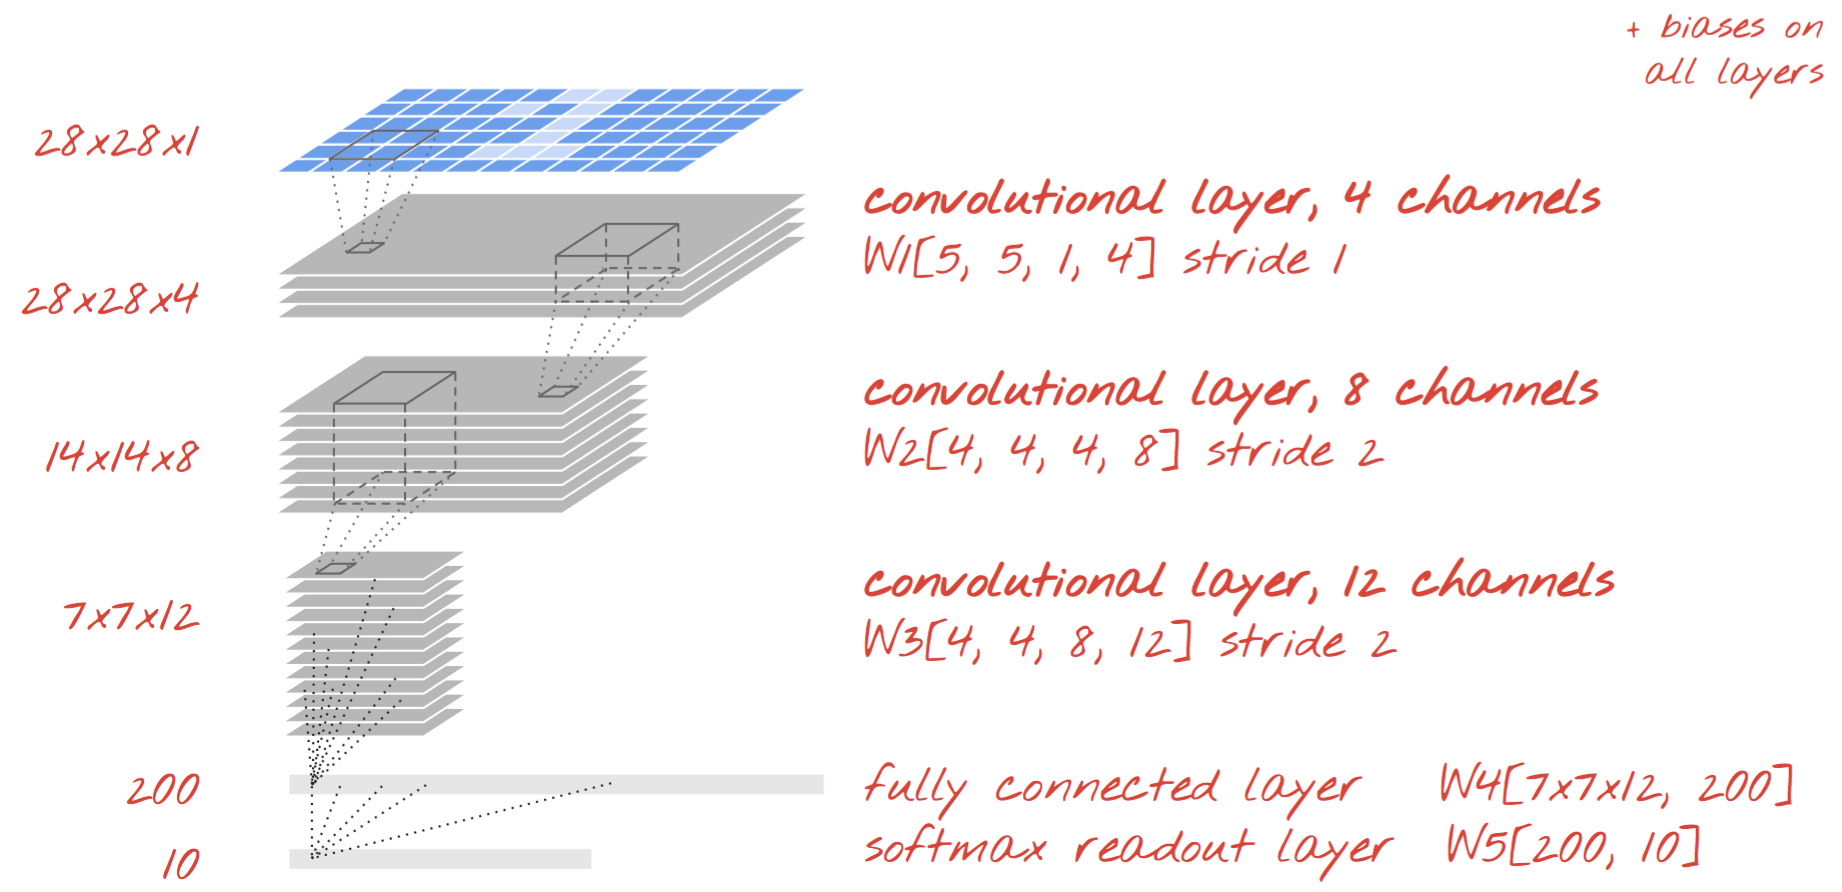
\includegraphics[width=0.9\textwidth]{figures/mnist-conv2d-1.png}
\caption{实现卷积神经网络}
 \label{fig:mnist-conv2d-1}
\end{figure}

使用\tf{}实现卷积网络,如下代码所示。

\begin{leftbar}
\begin{python}
K = 4 
L = 8
M = 12
N = 200

w1 = tf.Variable(tf.truncated_normal([5, 5, 1, K], stddev=0.1))
b1 = tf.Variable(tf.ones([K])/10)

w2 = tf.Variable(tf.truncated_normal([5, 5, K, L], stddev=0.1))
b2 = tf.Variable(tf.ones([L])/10)

w3 = tf.Variable(tf.truncated_normal([4, 4, L, M], stddev=0.1))
b3 = tf.Variable(tf.ones([M])/10)

w4 = tf.Variable(tf.truncated_normal([7 * 7 * M, N], stddev=0.1))
b4 = tf.Variable(tf.ones([N])/10)

w5 = tf.Variable(tf.truncated_normal([N, 10], stddev=0.1))
b5 = tf.Variable(tf.ones([10])/10)

y1 = tf.nn.relu(tf.nn.conv2d(
       x,  w1, strides=[1, 1, 1, 1], padding='SAME') + b1)
y2 = tf.nn.relu(tf.nn.conv2d(
       y1, w2, strides=[1, 2, 2, 1], padding='SAME') + b2)
y3 = tf.nn.relu(tf.nn.conv2d(
       y2, w3, strides=[1, 2, 2, 1], padding='SAME') + b3)

yy = tf.reshape(Y3, shape=[-1, 7 * 7 * M])
y4 = tf.nn.relu(tf.matmul(yy, w4) + b4)

logits = tf.matmul(y4, w5) + b5
y = tf.nn.softmax(logits)
\end{python}
\end{leftbar}

如\refig{mnist-conv2d-1-result}所示,经过$10^4$次训练,可以得到大约\percent{98.9}的准确率。

\begin{figure}[H]
\centering
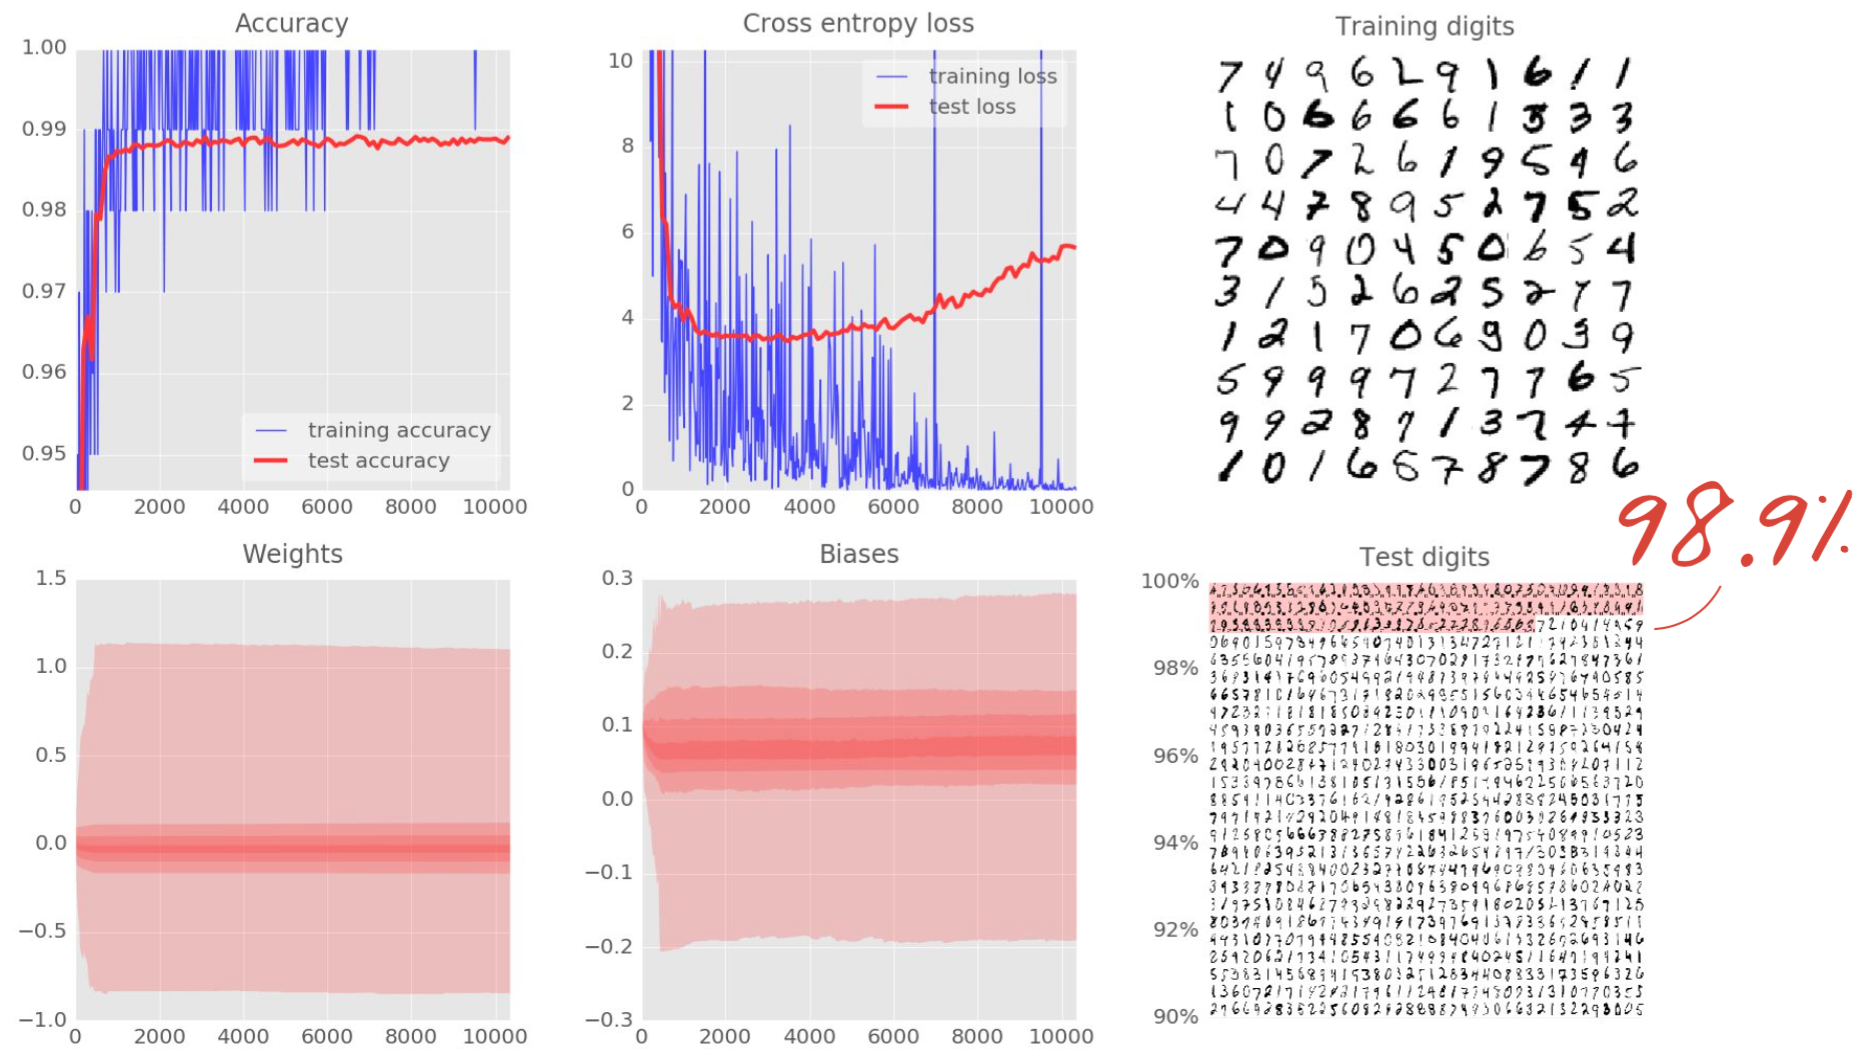
\includegraphics[width=0.9\textwidth]{figures/mnist-conv2d-1-result.png}
\caption{实现卷积网络:可以得到\percent{98.9}的准确率}
 \label{fig:mnist-conv2d-1-result}
\end{figure}

\subsection{增强卷积网络}

如\refig{mnist-conv2d-2}所示,保留之前的网络层次结构,构造了\ascii{3}个卷积层和\ascii{2}个全连接层。其中,中间隐藏层使用\ascii{ReLU}的激活函数,最后的输出层采用\ascii{softmax}的激活函数。

但是,相对于之前的卷积网络,使用了更多的通道提取更多的特征。同时,在全连接的隐藏层中实施\ascii{dropout}操作,增强网络的泛化能力。

\begin{figure}[H]
\centering
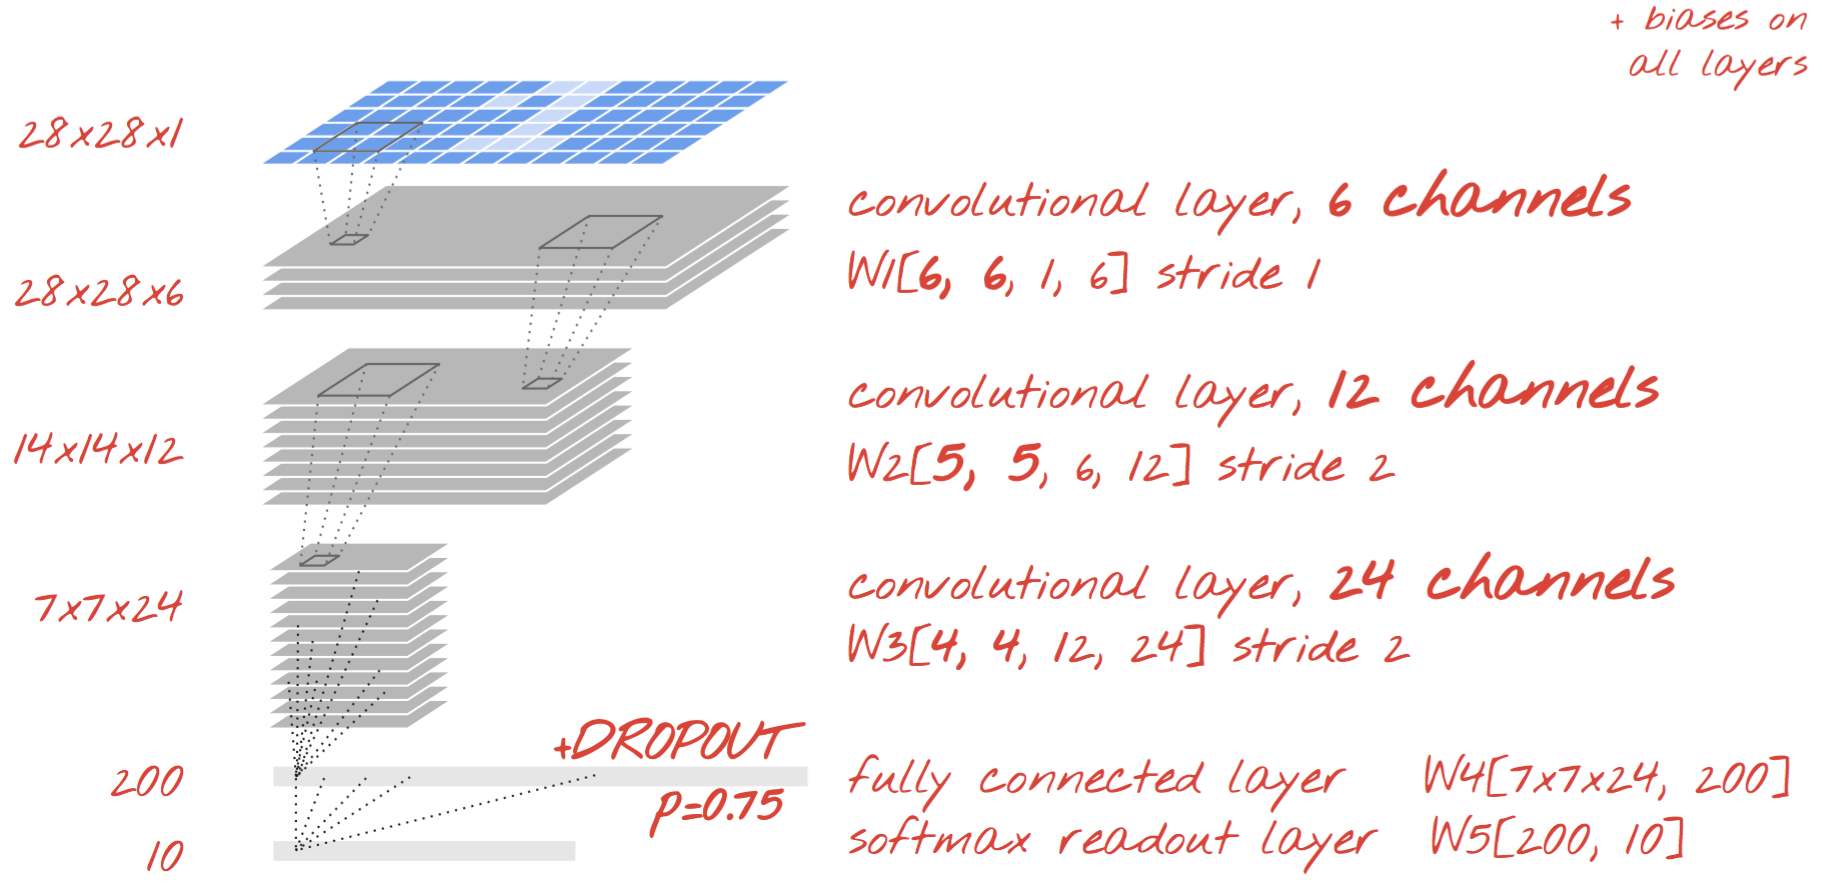
\includegraphics[width=0.9\textwidth]{figures/mnist-conv2d-2.png}
\caption{改善卷积神经网络}
 \label{fig:mnist-conv2d-2}
\end{figure}

使用\tf{}实现更大的卷积网络,如下代码所示。

\begin{leftbar}
\begin{python}
K = 6
L = 12
M = 24
N = 200

w1 = tf.Variable(tf.truncated_normal([6, 6, 1, K], stddev=0.1))
b1 = tf.Variable(tf.ones([K])/10)

w2 = tf.Variable(tf.truncated_normal([5, 5, K, L], stddev=0.1))
b2 = tf.Variable(tf.ones([L])/10)

w3 = tf.Variable(tf.truncated_normal([4, 4, L, M], stddev=0.1))
b3 = tf.Variable(tf.ones([M])/10)

w4 = tf.Variable(tf.truncated_normal([7 * 7 * M, N], stddev=0.1))
b4 = tf.Variable(tf.ones([N])/10)

w5 = tf.Variable(tf.truncated_normal([N, 10], stddev=0.1))
b5 = tf.Variable(tf.ones([10])/10)

y1 = tf.nn.relu(tf.nn.conv2d(
       x,  w1, strides=[1, 1, 1, 1], padding='SAME') + b1)
y2 = tf.nn.relu(tf.nn.conv2d(
       y1, w2, strides=[1, 2, 2, 1], padding='SAME') + b2)
y3 = tf.nn.relu(tf.nn.conv2d(
       y2, w3, strides=[1, 2, 2, 1], padding='SAME') + b3)

yy = tf.reshape(Y3, shape=[-1, 7 * 7 * M])
y4 = tf.nn.relu(tf.matmul(yy, w4) + b4)
y4d = tf.nn.dropout(y4, pkeep)

logits = tf.matmul(y4d, w5) + b5
y = tf.nn.softmax(logits)
\end{python}
\end{leftbar}

如\refig{mnist-conv2d-2-result}所示,经过$10^4$次训练,可以得到大约\percent{99.3}的准确率。

\begin{figure}[H]
\centering
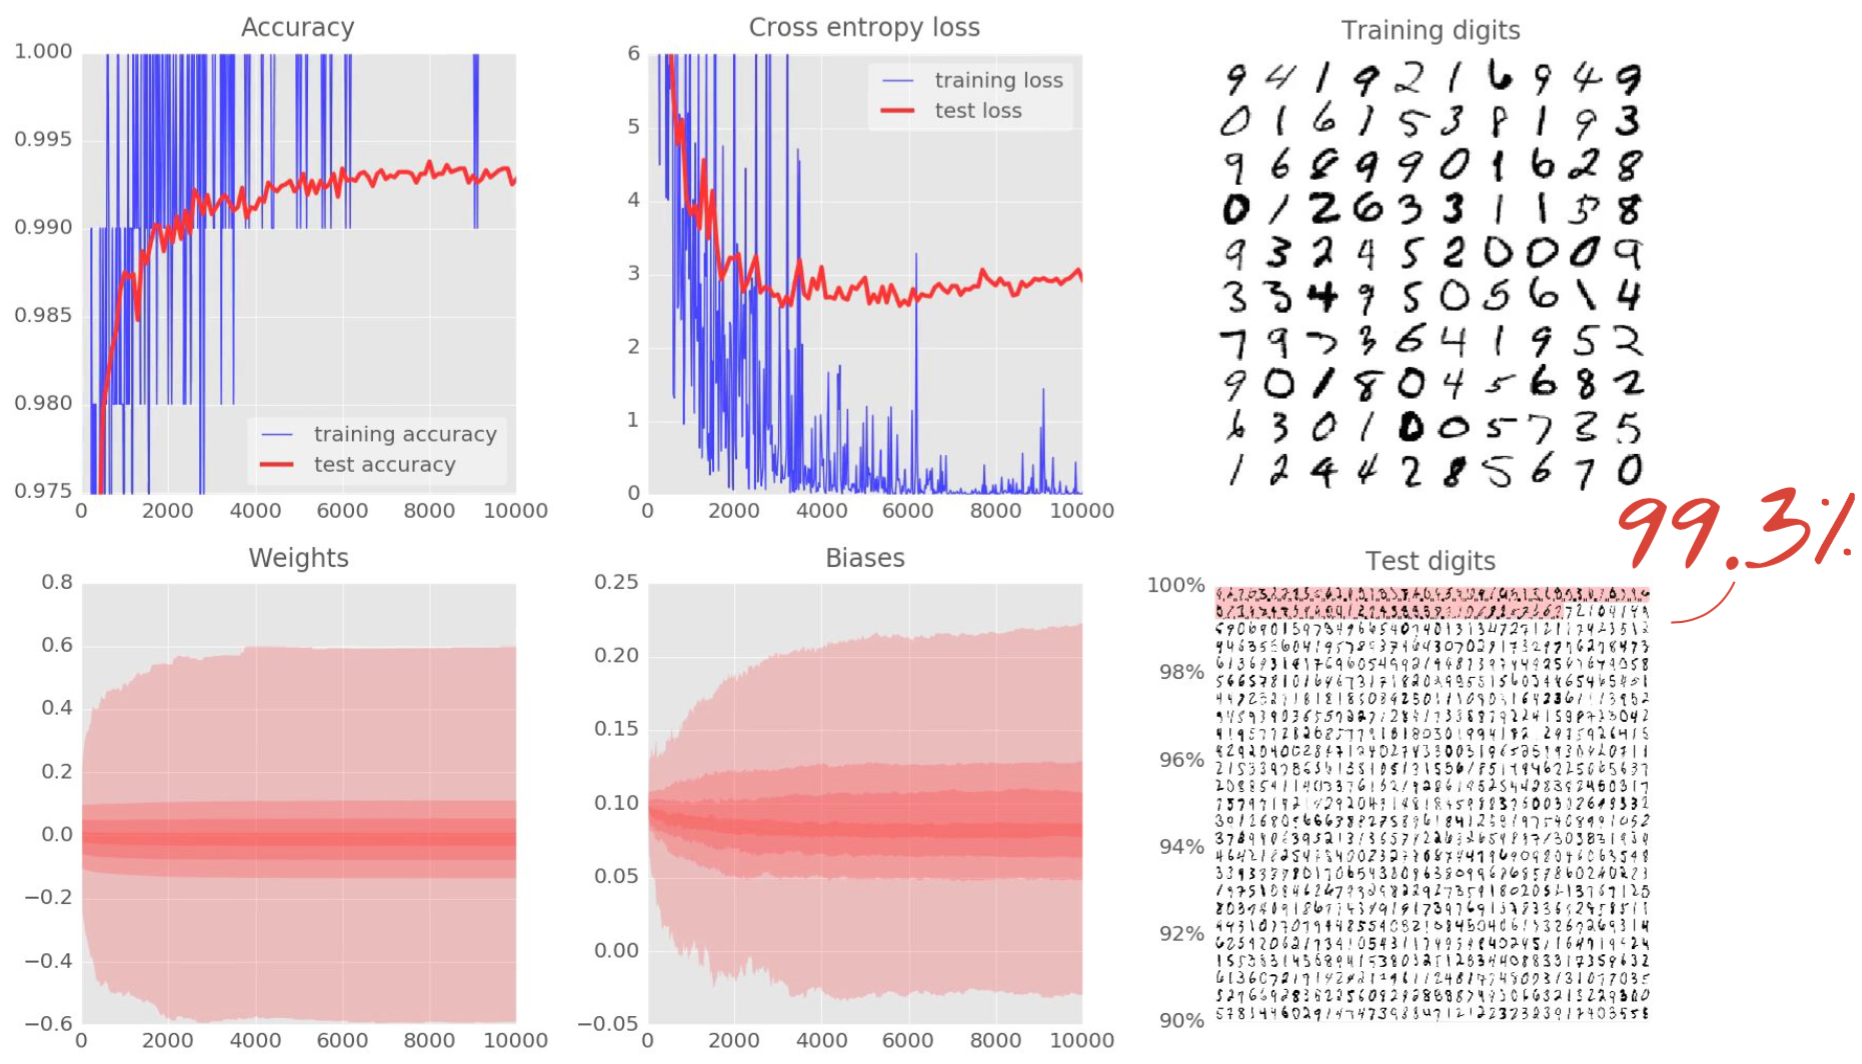
\includegraphics[width=0.9\textwidth]{figures/mnist-conv2d-2-result.png}
\caption{增强卷积网络:可以得到\percent{99.3}的准确率}
 \label{fig:mnist-conv2d-2-result}
\end{figure}

同时,相对于之前实现的卷积网络,过拟合问题得到了明显地改善,如\refig{mnist-conv2d-3-result}所示。

\begin{figure}[H]
\centering
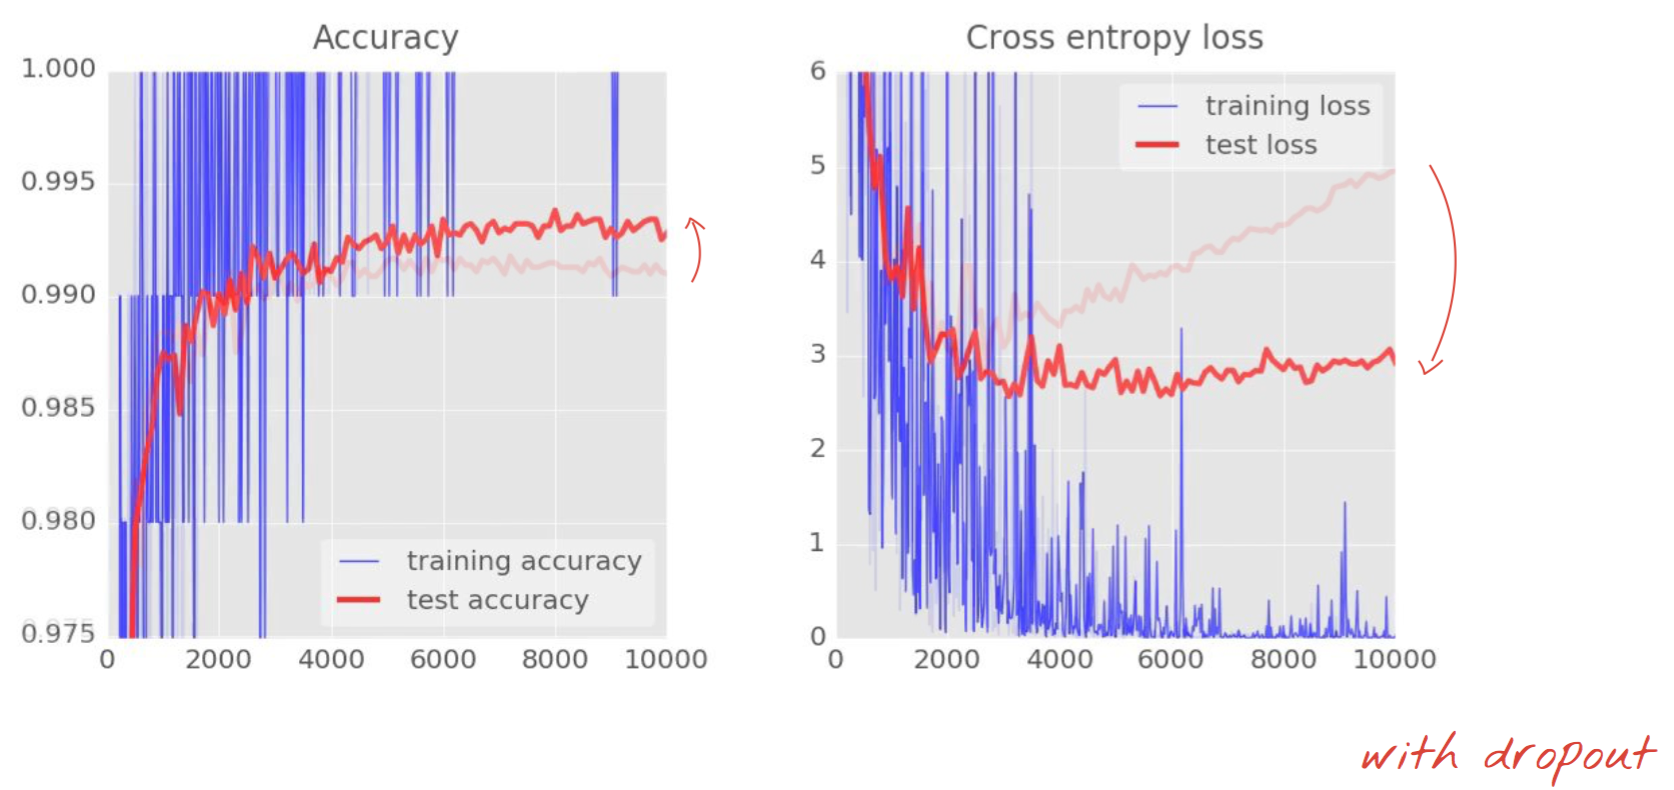
\includegraphics[width=0.9\textwidth]{figures/mnist-conv2d-3-result.png}
\caption{增强卷积网络:过拟合问题明显改善}
 \label{fig:mnist-conv2d-3-result}
\end{figure}

\end{content}